\chapter{开放环境中的细粒度主机属性发现}\label{chap:First_Point}
本章提出了一种基于协议字段特征和流统计特征的主机属性识别技术,用于在开放的动态网络中精准地识别主机的多维属性。本章首先概述该工作的背景意义、技术原理和思路流程,然后分别介绍识别技术中的关键环节,最终展示识别技术的实验效果。

\section{引言}
%保障网络安全最大的挑战之一就是及时发现漏洞,而绝大部分安全漏洞和隐患都与细粒度的主机属性息息相关。此外,识别网络中主机的多维细粒度属性还可以帮助网络运营者有效地进行网络管理、网络资源分配、网络服务质量优化。探测目标主机的相关属性一般分为主动和被动两种方式,而由于入侵检测技术的成熟,主动探测技术的局限性越来越明显,本章将介绍一种被动探测技术,可以精准、快速的识别加密网络中的细粒度主机属性。

尽管RFC文档已经对TCP/IP协议栈的规范进行了统一,但是不同厂商的软件开发者在实际开发和更新操作系统、浏览器等软件的过程中,由于缺乏协商,对网络协议栈的初始化参数进行了不同的设置。这一现象造成了不同属性的主机在网络会话过程中,存在明显的协议字段参数差异和流统计数据差异,称为TCP/IP协议栈指纹。本章方法以TCP/IP协议栈指纹为基础,结合以LightGBM为代表的机器学习模型,对当前主流的操作系统和浏览器进行识别。

如图3.1所示,本章方法首先从网络中采集TLS加密会话,以双向流为单位,提取每条TLS流的TCP/IP协议字段特征、TLS协议字段特征以及流统计特征,在经过数据处理后作为机器学习模型的输入,最终得到多维主机属性。

\begin{figure}[!htbp]
    \centering
    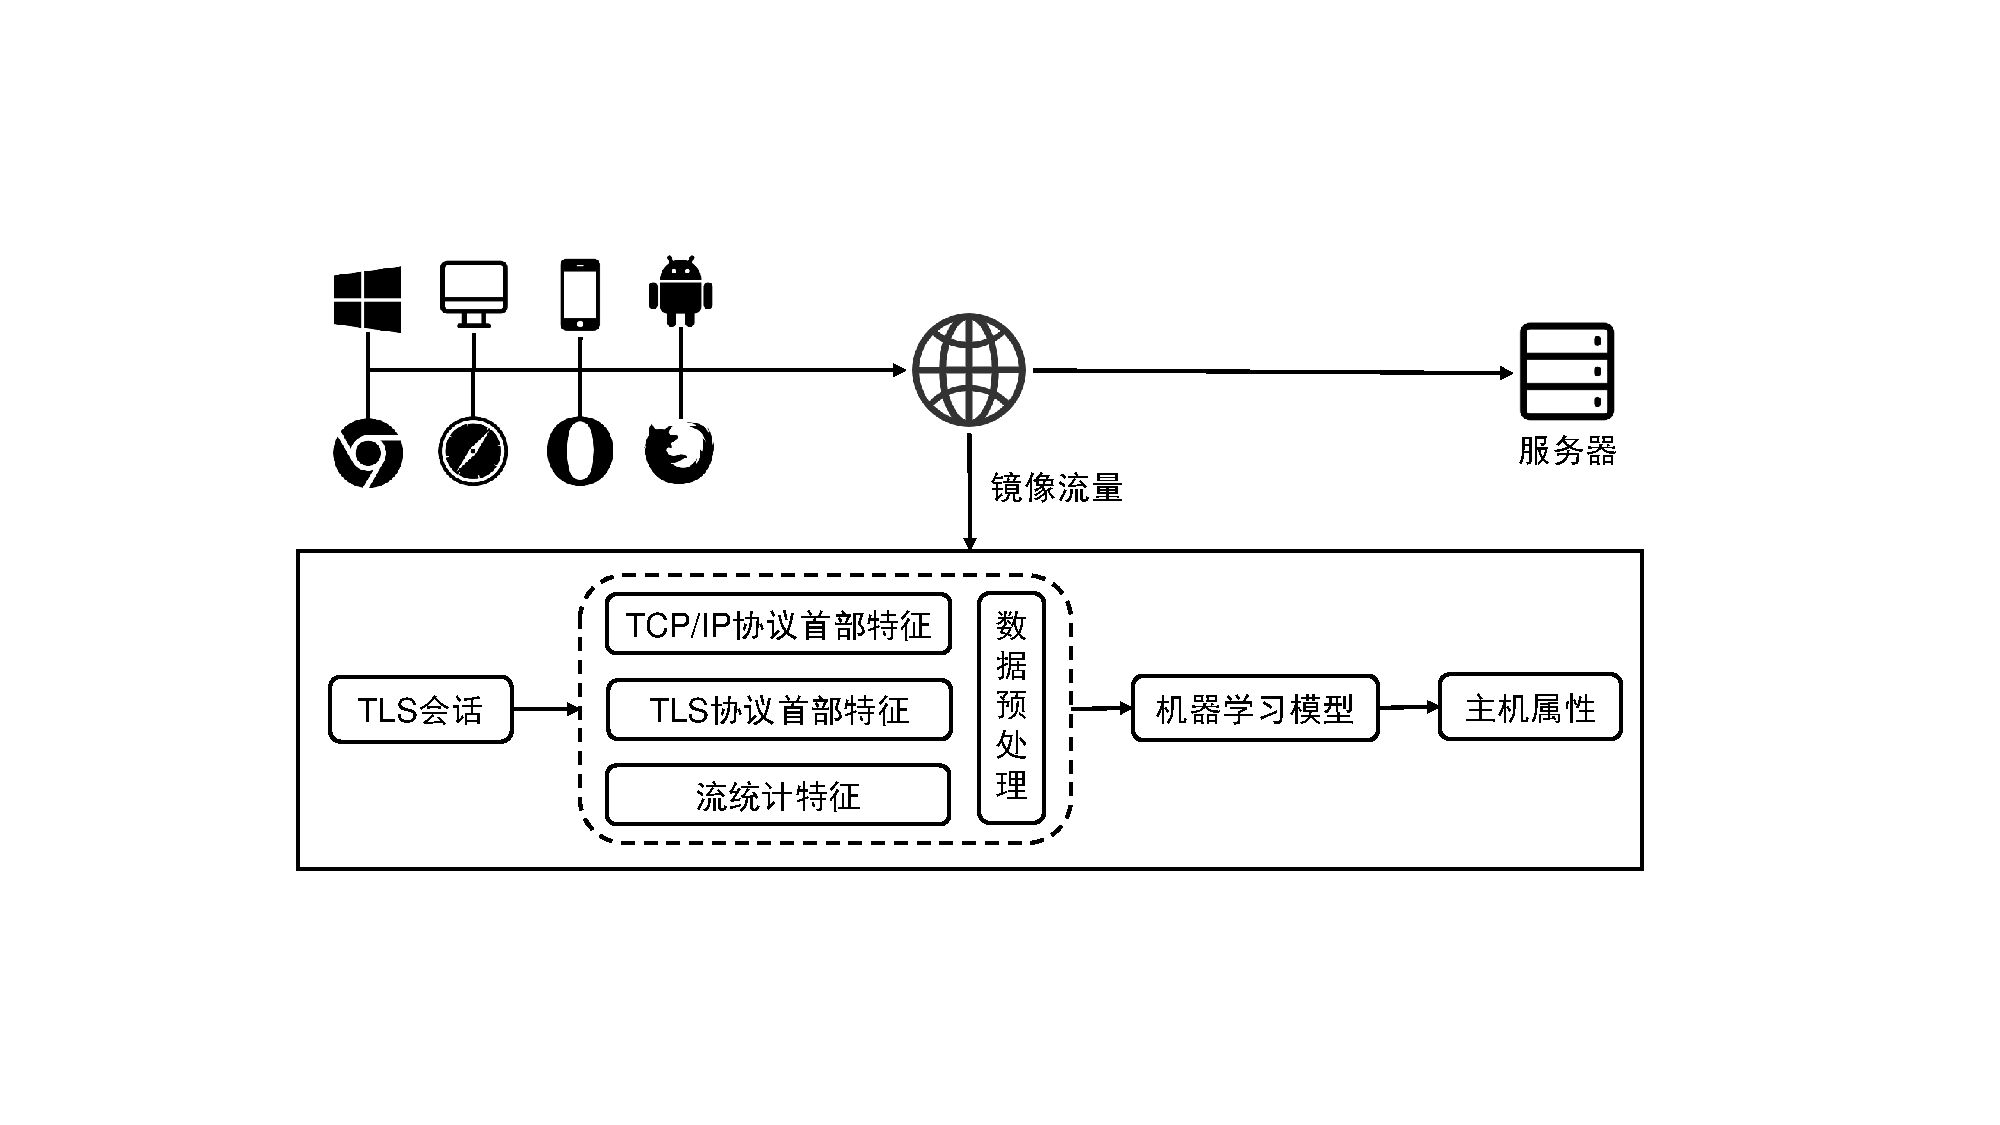
\includegraphics[width=0.9\textwidth]{研究点1结构}
    \bicaption{开放环境中的细粒度主机属性发现技术}{Fine-grained host attribute discovery technology in an open environment}
\end{figure}

\section{特征工程}

在流量识别场景中,单向网络流通常指在一段时间内,具有相同五元组<源地址,目的地址,源端口,目的端口,传输协议类型>的所有数据包形成的包序列。双向网络流由同一时间段内源目地址可互换的单向流组成。本节将介绍以双向流为单位的协议字段特征和流统计特征的提取方法。

\subsection{协议字段特征}

TCP/IP协议栈采用五层网络模型结构,自下向上分别为:物理层,数据链路层、网络层、传输层和应用层。在一次完整的TLS会话中,网络层的主要协议为IP协议,传输层的主要协议为TCP协议。TCP协议是面向连接的协议,一般通过交互三个数据包完成连接的建立。本章从由客户端发往服务端的第一个数据包即TCP SYN包中提取IP协议首部字段和TCP协议首部字段,从TLS Client Hello包中提取TLS协议首部字段。如表3.1所示,本章方法分别从IP协议、TCP协议以及TLS协议首部中提取3维特征、4维特征、6维特征,组成共计13维特征的TCP/IP协议栈指纹。

\begin{table}[!htbp] 
    \bicaption{协议字段特征}{Protocol field features}
    \centering
    \footnotesize
    \setlength{\tabcolsep}{20pt}
    \renewcommand{\arraystretch}{1}
\begin{tabular}{lll}
\toprule
协议 & 特征 & 说明 \\ \hline
\multirow{3}{*}{IP} & time\underline{~~}to\underline{~~}live & 生存时间 \\ 
& total\underline{~~}length & IP包长\\ 
& fragment\underline{~~}flag & 分片标志\\ \hline
\multirow{4}{*}{TCP} & window\underline{~~}size & TCP窗口大小 \\ 
 & window\underline{~~}scale & 窗口缩放因子 \\ 
 & maximum\underline{~~}segment\underline{~~}size & 最大报文长度 \\ 
 & option\underline{~~}type\underline{~~}codes\underline{~~}sequence & 可选项类型序列 \\ \hline
\multirow{6}{*}{TLS} & version & 版本 \\ 
 & dxtensions\underline{~~}length & 扩展长度 \\ 
 & cipher\underline{~~}suite\underline{~~}codes\underline{~~}sequence & 密钥算法套件序列 \\ 
 & extension\underline{~~}type\underline{~~}codes\underline{~~}sequence & 扩展类型序列 \\ 
 & supported\underline{~~}group\underline{~~}codes\underline{~~}sequence & 支持加密组件序列 \\ 
 & ALPN\underline{~~}codes\underline{~~}sequence & 应用层协议协商序列 \\ 
\bottomrule
%random\underline{~~}state & 随机种子 & 6 \\
\end{tabular}
\end{table}

IP报文通常由首部和载荷组成,首部长度可变,通常为20字节,可以根据不同的需要加入各种可选项部分。IP首部的一般格式如图3.2所示,其中,本章方法所提取的IP协议首部参数主要为生存时间,总长度以及分片标志。

\begin{figure}[!htbp]
    \centering
    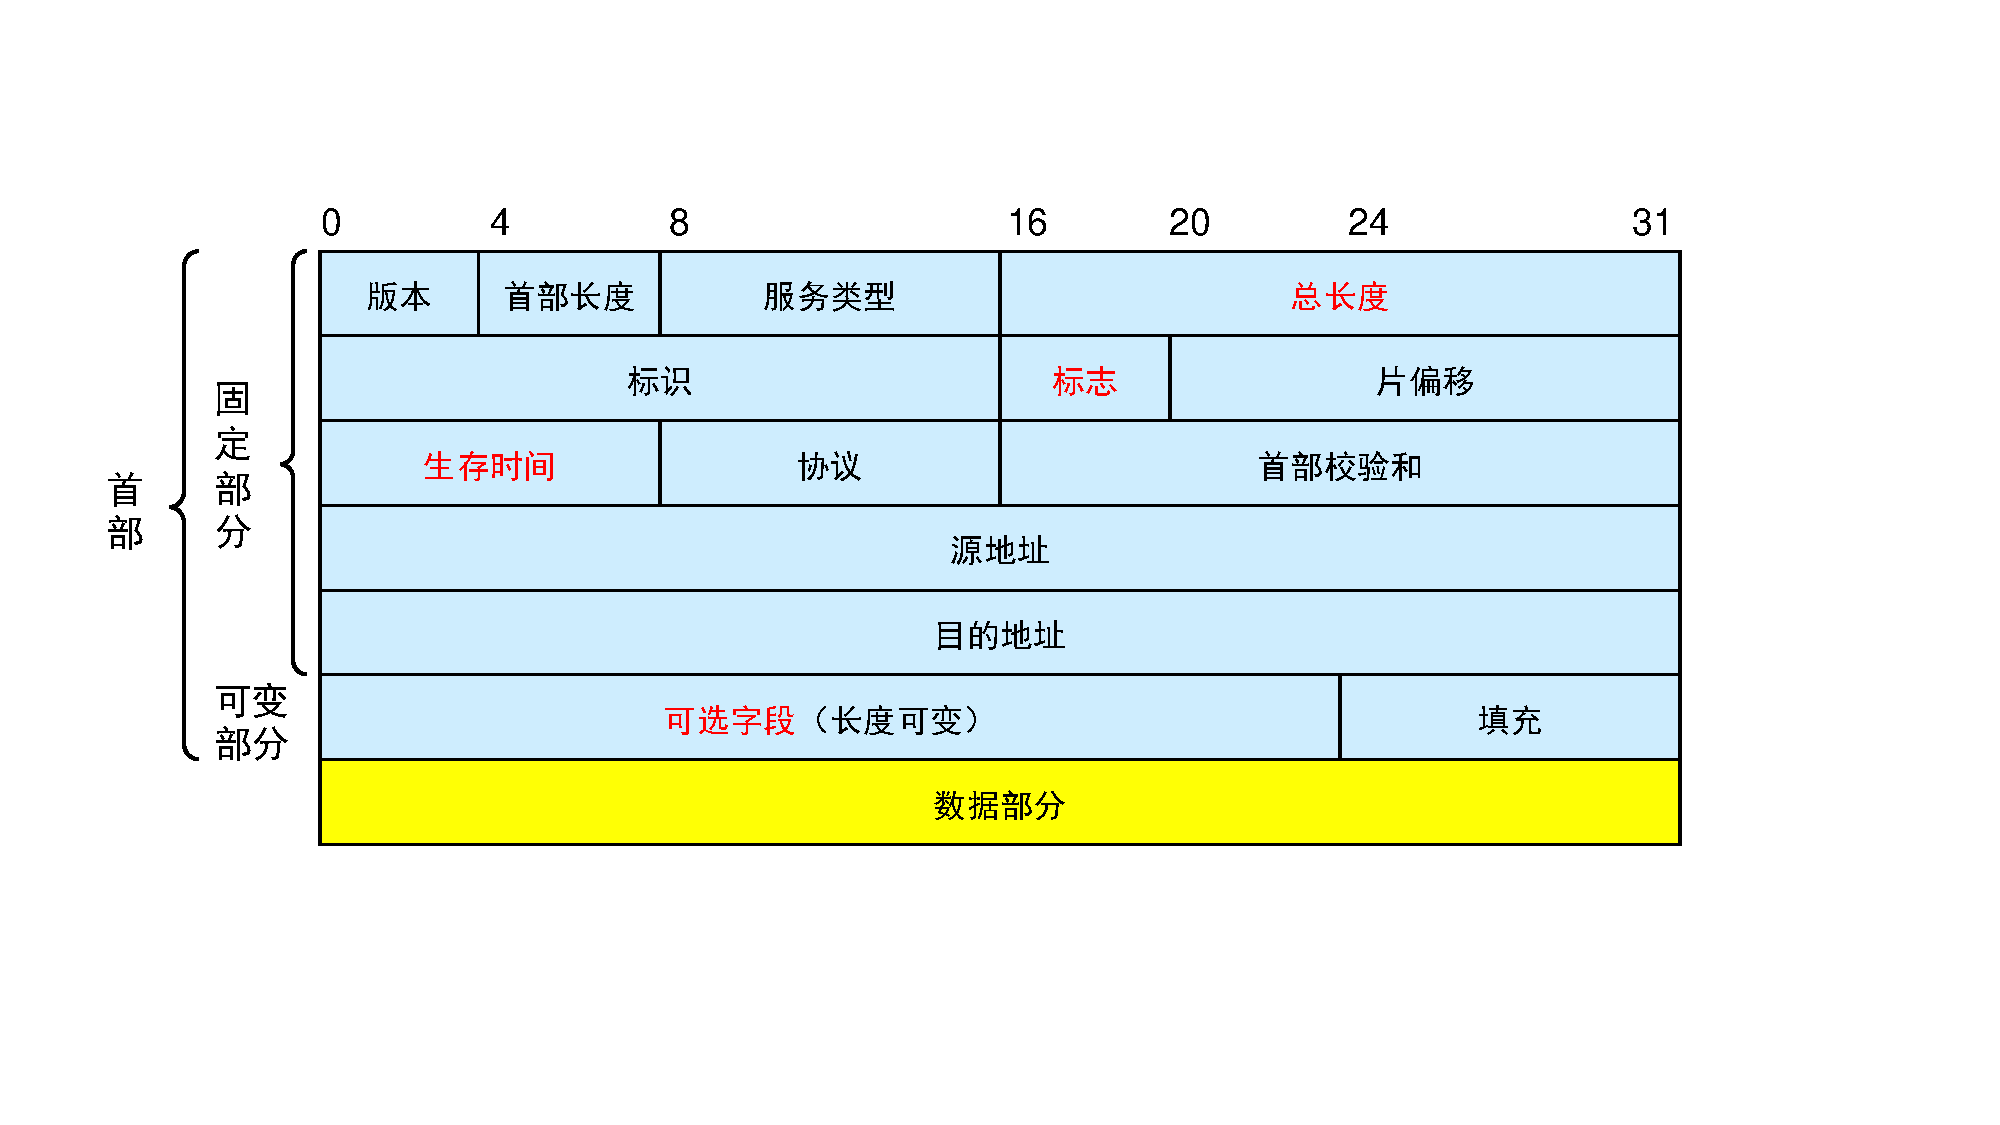
\includegraphics[width=0.9\textwidth]{3-2}
    \bicaption{IP报文格式}{IP protocol format}
    \label{fig:3-2}
\end{figure}

\begin{itemize}
\item 
生存时间(TTL):IP报文所允许通过的路由器的最大数量。每经过一个路由器,TTL减1,当为0时,路由器将该数据报丢弃。TTL字段是由发送端初始设置一个8bit字段,记录了报文在网络中的存活时间,各类操作系统的TTL初始值不同。
\item 
总长度:IP报文的总长度,是报头的长度和载荷的长度之和。
\item 
分片标志:1bit字段,1表示报文不分片,0表示分片。
\end{itemize}

\begin{figure}[!htbp]
    \centering
    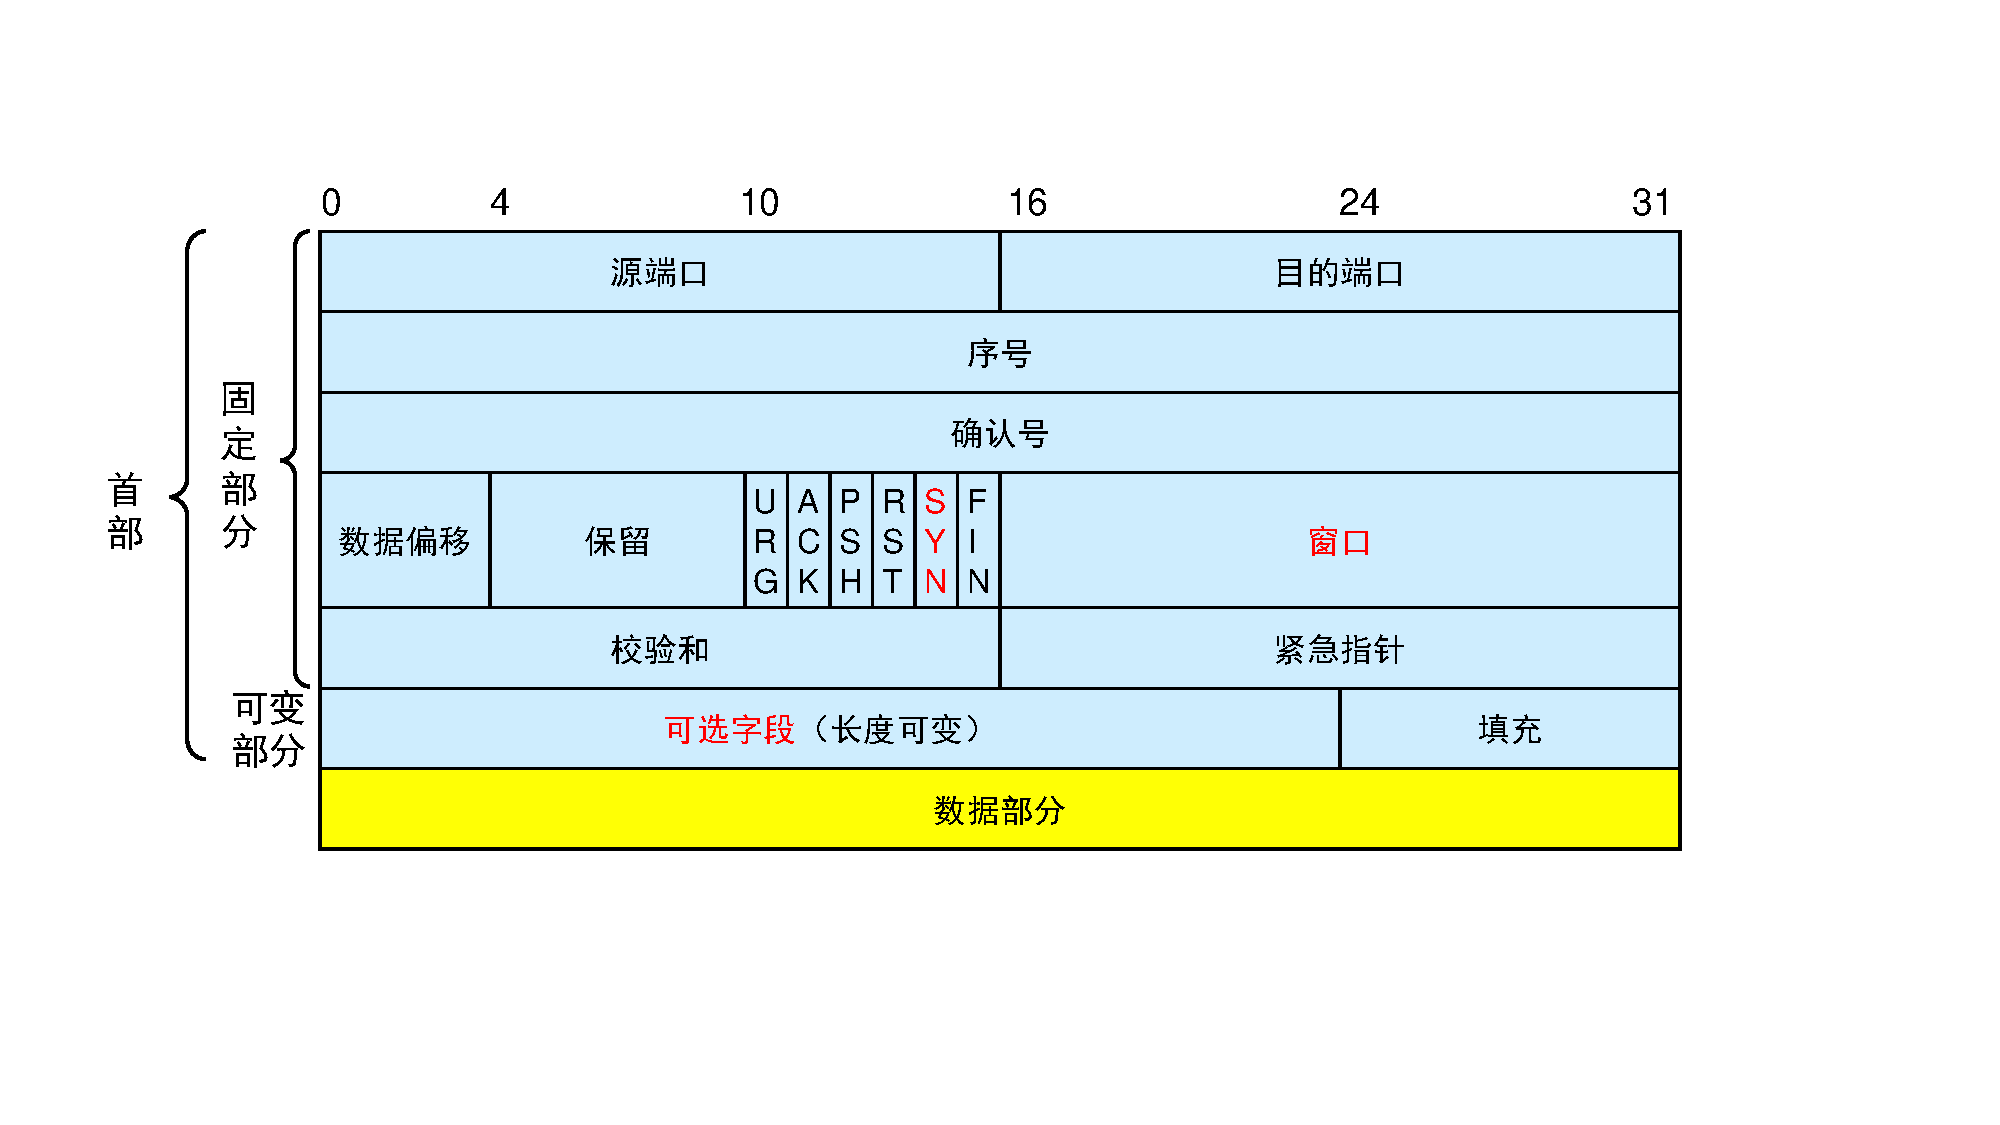
\includegraphics[width=0.9\textwidth]{3-3}
    \bicaption{TCP报文格式}{TCP protocol format}
    \label{fig:3-3}
\end{figure}

TCP报文同样由首部和载荷组成,首部长度一般为20字节,可以扩展不同的可选项部分。TCP首部的一般格式如图3.3所示。其中,本章方法所提取的TCP协议首部参数主要为窗口大小,窗口缩放因子,最大报文长度以及可选项类型序列。

\begin{itemize}
\item 
窗口大小:用来告知对端本地的缓存大小,以此控制对端发送数据的速率,从而达到流量控制的目的。窗口大小为一个16bit字段,因而最大为65535。
\item 
窗口缩放因子:用于提高传输窗口的上限。
\item 
最大报文长度:每一个TCP报文段中数据字段的最大长度。其值太大或太小都不合适,太小会使得数据传输效率很低,太大会增加网络丢包的可能性,增大网络开销。
\item
可选项类型序列:按照字节顺序解析TCP SYN包的可选项字段,从中提取出每一个可选项子字段的类型,并按照一定的编码方式将其转换为类型码,便可得到有序的类型码序列。在本章方法的编码方式中,将NOP类型记作0,最大报文长度类型记作1,窗口缩放因子类型记作2,选择确认项类型记作3,时间戳类型记作4,其他类型记作5。最终得到的类型序列一般形式为$opt\underline{~~}seq=< o_{1},o_{2},o_{3},...,o_{n} >,o_{i}∈[0,5]$。
\end{itemize}

\begin{figure}[!htbp]
    \centering
    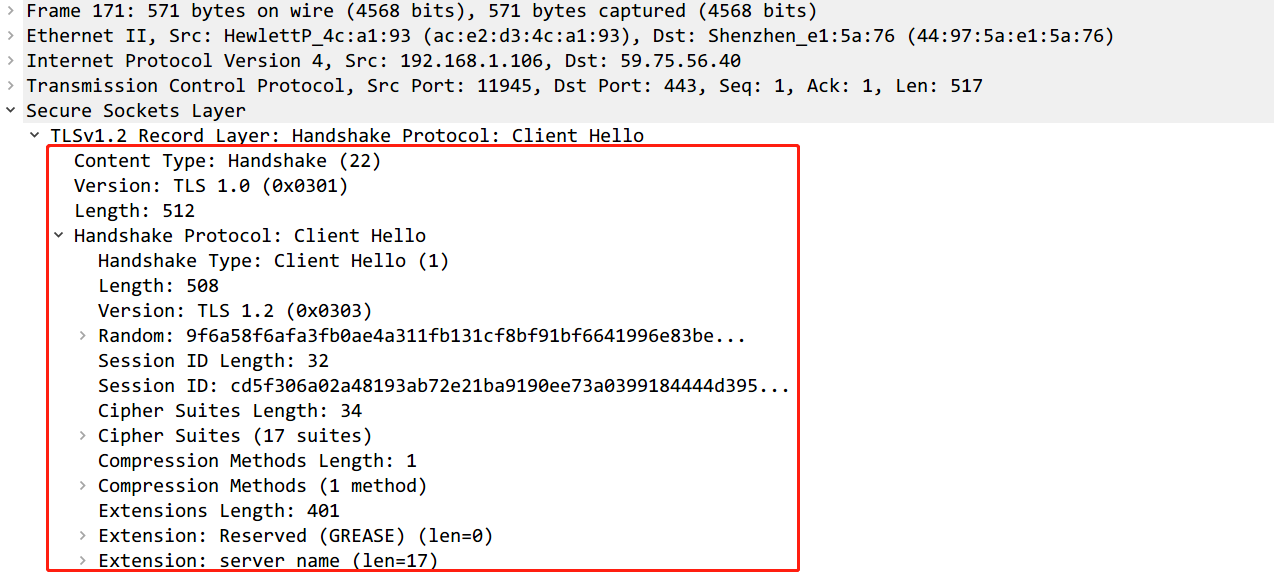
\includegraphics[width=0.9\textwidth]{3-4}
    \bicaption{TLS报文格式}{TLS protocol format}
    \label{fig:3-4}
\end{figure}
TLS Client Hello报文是TLS建立会话的第一个数据报文,本章方法提取的报文首部字段主要有协议版本,密钥算法套件序列,扩展长度,扩展类型序列,支持加密组件序列以及应用层协议协商状态码序列。其报文格式如图3.4所示。

\begin{itemize}
\item 
协议版本:表示客户端支持的最佳TLS协议版本。
\item 
密钥算法套件序列:由客户端支持的所有密钥算法套件组成的状态码序列。加密套件包含客户端能够支持的加密方式、算法等信息。不同的加密套件性能存在差异,同时会产生不同的TLS交互报文。
\item 
扩展长度:TLS协议的扩展部分长度。
\item 
扩展类型序列:TLS协议的扩展部分由任意数量的不同扩展组成。每一类扩展都有一个独特的类型码,按字节顺序解析扩展部分的所有扩展,即可得到扩展类型序列。
\item 
支持加密组件序列:按字节顺序解析,得到Supported Groups扩展字段中的类型码序列。
\item 
应用层协议协商状态码序列:按字节顺序解析,得到Application Layer Protocol Negotiation扩展字段中的类型码序列。
\end{itemize}

\subsection{流统计特征}

流统计特征可以轮廓性地描述不同属性的主机在网络通信过程中的差异。以每条流前50个包的长度序列和时间间隔序列为基础,分别提取网络流在空间、时间以及速率等三个维度的统计特征。空间特征主要包括总包数、总字节数、包长均值、包长均方差、包长直方图分布和包长马尔可夫状态转移矩阵等。时间特征主要包括间隔均值、间隔均方差、间隔直方图分布和间隔马尔可夫状态转移矩阵等。速率特征主要包括包数吞吐量均值、字节数吞吐量均值以及传输峰值分布等。

\begin{itemize}
\item 
包长直方图分布:假设IP协议的最大传输单元为1500字节,设置组数为10,组距为150字节。根据包长序列统计前50个数据包的包长在每个分组中的频数,可得到长度为10的包长直方图分布。
\item 
间隔直方图分布:类似包长直方图分布,以毫秒为单位,将包到达时间间隔分为10组,组距为100毫秒,其中最后一组的组距为[ 900, Inf )。根据包到达时间间隔序列统计其在每个分组中的频数,可得到长度为10的间隔直方图分布。
\item 
包长马尔科夫状态转移矩阵:以包长直方图分布为基础,对每个分组按从小到大分配状态码1到10,根据包长在直方图中的分布便可得到每个包对应的包长状态码。初始化一个10*10的全0矩阵,行号表示前一个数据包的包长状态,列号表示后一个数据包的包长状态,依次统计前50个包的包长状态转移概率,可得到包长序列的马尔科夫状态转移矩阵。
\item 
间隔马尔科夫状态转移矩阵:同样,以间隔直方图分布为基础,对每个分组按从小到大分配状态码1到10,根据相邻数据包的时间间隔在直方图中的分布便可得到对应的间隔状态码。初始化一个10*10的全0矩阵,行号表示间隔序列中前一个间隔状态,列号表示后一个间隔状态,依次统计前50个包的时间间隔状态转移概率,可得到间隔马尔科夫状态转移矩阵。
\end{itemize}

\section{机器学习模型构建}

无论在主动或者被动的主机属性发现技术中,传统方法一般是首先获取TCP/IP协议字段初始值以生成指纹,然后将获得的指纹与预先生成的已知主机属性指纹库中的指纹进行对比,当待识别指纹与已知指纹完全匹配时,便可得到具体的主机属性。传统方法属于静态方法,优点是识别速度快,缺点是无法识别不在指纹库中的未知指纹。为了克服以上缺陷,本章将构建五类经典的机器学习模型用于识别所有指纹的主机属性,提高识别方法的灵活性、准确性和鲁棒性。这五类机器学习模型分别为逻辑回归(Logistics Regression, LR)模型、最近邻居(K-nearest Neighbour, KNN)模型、随机森林(Random Forest, RF)模型、XGBoost模型以及LightGBM模型。

\subsection{逻辑回归模型}

逻辑回归算法是基于线性回归算法的改进算法,也是解决二分类问题的首选方法,在将其推广到多项逻辑回归算法后,可用于多分类任务。与线性回归模型相似,LR模型首先计算每个输入特征的权重,即系数值。然后利用Logistic函数对线性输出值进行非线性变换,使得最终的预测输出值介于0到1之间。模型优点是计算成本小,易于理解和实现。缺点是易出现欠拟合问题,分类精度可能不高。结合网格搜索策略和交叉验证法,逻辑回归模型的最优参数组合如表3.2所示。

\begin{table}[!htbp] 
    \bicaption{逻辑回归模型参数选择}{Logistic regression model parameter selection}
%    \label{tab:sample}
    \centering
    \footnotesize
    \setlength{\tabcolsep}{20pt}
    \renewcommand{\arraystretch}{1.2}
\begin{tabular}{lll}
\toprule
参数 & 含义 & 取值 \\ \hline
penalty & 正则项选择 & l1 \\ 
solver & 损失函数的优化方法 & liblinear \\ 
max\underline{~~}iter & 算法收敛的最大迭代次数 & 4000\\ 
multi\underline{~~}class & 多分类方法 & multinomial \\ 
%random\underline{~~}state & 随机种子 & 6 \\
\bottomrule
\end{tabular}
\end{table}

\subsection{最近邻居模型}

KNN模型是一种用于分类和回归的非参数统计方法。算法的原理是假设相同类别样本之间的相似度更高,可以通过计算与已知类别样本的相似度,来评估未知类别样本可能的分类,是一种基于实例的学习算法。参数K的取值、样本之间的距离度量算法以及分类决策规则是KNN算法的三要素。KNN模型的优点是精度高,对异常值不敏感。缺点是计算复杂度和空间复杂度较高。最近邻居模型的最优参数组合如表3.3所示,其中K值为7。

\begin{table}[!h] 
    \bicaption{最近邻居模型参数选择}{Nearest neighbor model parameter selection}
%    \label{tab:sample}
    \centering
    \footnotesize
    \setlength{\tabcolsep}{20pt}
    \renewcommand{\arraystretch}{1}
\begin{tabular}{lll}
\toprule
参数 & 含义 & 取值 \\ \hline
n\underline{~~}neighbors & KNN模型中的k值 & 7 \\ 
weights & 每个样本的近邻样本的权重 & distance \\ 
algorithm & 限定半径最近邻法使用的算法 & auto\\ 
metric & 距离度量算法 & minkowski \\ 
\bottomrule
\end{tabular}
\end{table}

\subsection{随机森林模型}

决策树是机器学习中的基础模型,它表示样本类别与样本属性值之间的一种映射关系。树中每个节点表示某类样本,每个分叉路径代表某个可能的属性值,而每个叶节点则表示从根节点到叶节点所需路径对应的属性值集合。RF模型作为基于Bagging思想的集成学习算法,是一种包含多个决策树的分类模型,其输出类别由所有树输出的类别众数而定,因此抗过拟合能力较强。RF模型的最优参数组合如表3.4所示,决策树的生长策略基于Gini系数。

\begin{table}[!h] 
    \bicaption{随机森林模型参数选择}{Random forest model parameter selection}
%    \label{tab:sample}
    \centering
    \footnotesize
    \setlength{\tabcolsep}{20pt}
    \renewcommand{\arraystretch}{1}
\begin{tabular}{lll}
\toprule
参数 & 含义 & 取值 \\ \hline
n\underline{~~}estimators & 决策树的数量 & 1500 \\ 
max\underline{~~}features & 特征子集中的特征数目 & auto \\ 
%max\underline{~~}depth & 树的最大深度 & None\\ 
min\underline{~~}samples\underline{~~}split & 节点最小分割的样本数 & 3 \\
criterion & 树的切分策略 & gini\\ 
bootstrap & 是否有放回的采样 & true\\ 
%random\underline{~~}state & 随机种子 & 5 \\
\bottomrule
\end{tabular}
\end{table}

\subsection{XGBoost模型}
XGBoost模型是一种提升树集成模型,属于梯度提升树(GBDT)模型的范畴,基学习器一般选择CART回归树模型,但也可以选择其它类型的模型如逻辑回归算法等。GBDT算法的基本思想是让新的基学习器去拟合前面学习器的偏差,从而不断将加法模型的偏差降低。相对比GBDT算法,XGBoost模型将目标函数进行了二阶泰勒展开,同时加入更多的正则项以及其他改进,显著提升了模型效果和性能。优点是分类精度非常高,缺点是计算代价较大。XGBoost模型的最优参数组合如表3.5所示。

\begin{table}[!h] 
    \bicaption{XGBoost模型参数选择}{XGBoost model parameter selection}
%    \label{tab:sample}
    \centering
    \footnotesize
    \setlength{\tabcolsep}{20pt}
    \renewcommand{\arraystretch}{1.2}
\begin{tabular}{lll}
\toprule
参数 & 含义 & 取值 \\ \hline
booster & 基学习器 & gbtree \\ 
early\underline{~~}stopping\underline{~~}rounds & 早期停止迭代次数 & 1500 \\ 
eta & 学习率 & 0.15 \\ 
min\underline{~~}child\underline{~~}weight & 叶子节点最小权重的和 & 0.7 \\ 
max\underline{~~}depth & 每棵树的最大深度 & 9 \\
subsample & 每棵树的随机样本采样比例 & 0.4 \\ 
colsample\underline{~~}bytree & 每棵树随机采样的特征比例 & 0.7 \\ 
alpha & L1正则化项的权重 & 0.5 \\ 
%seed & 随机种子 & 5 \\
\bottomrule
\end{tabular}
\end{table}

\subsection{LightGBM模型}
与XGBoost模型相同,LightGBM模型也是一种提升树集成模型,属于梯度提升树模型的范畴。但由于采用了Histogram算法,LightGBM模型比XGBoost模型更强大、速度更快。Histogram算法的基本思想是先把连续的浮点特征值离散化成k个整数,同时构造一个宽度为k的直方图。在遍历数据的时候,根据离散化后的值作为索引在直方图中累积统计量,当遍历完一次数据后,直方图便累积了需要的统计量,然后根据直方图的离散值,遍历寻找最优的分割点。该算法大幅降低了模型的内存消耗,显著提升了计算性能。此外,LightGBM模型采用带有深度限制的叶子生长算法代替了传统的决策树生长策略,防止过拟合现象的出现。而且通过优化对类别特征的支持,使得输入特征无需进行One-Hot编码处理。表3.6展示了LightGBM模型经过调参后的最优参数组合。

\begin{table}[!htbp] 
    \bicaption{LightGBM模型参数选择}{LightGBM model parameter selection}
%    \label{tab:sample}
    \centering
    \footnotesize
    \setlength{\tabcolsep}{20pt}
    \renewcommand{\arraystretch}{1}
\begin{tabular}{lll}
\toprule
参数 & 含义 & 取值 \\ \hline
learning\underline{~~}rate & 学习率 & 0.05 \\ 
boosting\underline{~~}type & 模型所用算法 & gbdt \\ 
%application & 模型用途 & multiclass \\ 
max\underline{~~}depth & 每棵树的最大深度 & 10 \\ 
num\underline{~~}leaves & 叶子节点数 & 512 \\ 
max\underline{~~}bin & bin的最大数量 & 500 \\ 
%min\underline{~~}data\underline{~~}in\underline{~~}leaf & 叶子节点中最小样本数 & 20 \\ 
num\underline{~~}boost\underline{~~}round & 迭代次数 & 500 \\ 
\bottomrule
\end{tabular}
\end{table}

\section{数据集构建}

本文于2019年5月6日到2019年5月10日持续五天在中国科技网中采集了约645万条网络流数据(包含了约96万台客户端主机发起的117万次HTTP会话和528万次TLS会话),称为原始数据集。由于主机属性发现任务属于监督学习任务,而获取的原始TLS会话数据缺少主机属性标签,因此本文采集了HTTP会话数据用于对TLS会话数据的属性标注。

\subsection{属性标注} 

在HTTP会话的请求报文中,通常存在一个首部字段User-Agent,它是一个特殊字符串,作用是使得服务器能够识别客户端主机的各种标识信息,如操作系统类型及版本、浏览器类型及版本、浏览器语言等,如图3.5所示。因此可利用HTTP报文的User-Agent字段对TLS会话数据集进行属性标注。

\begin{figure}[!h]
    \centering
    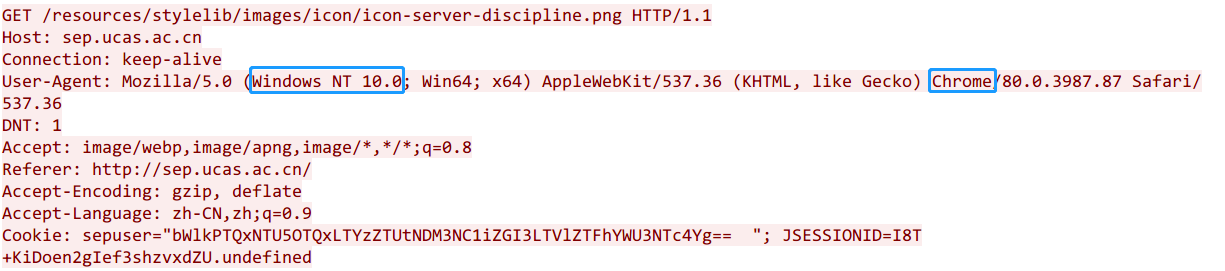
\includegraphics[width=0.9\textwidth]{3-5}
    \bicaption{HTTP协议请求报文中的User-Agent字段}{User-Agent field in HTTP request packet}
\end{figure}

\vbox{}

对于TLS会话数据集中的所有客户端IP地址,通过解析其发送的HTTP请求报文,可得到该IP地址对应的主机属性,并以键值对的形式将以上信息存储到一个主机属性标签字典中。当得到所有客户端IP的主机属性后,便完成了该字典的创建。然后通过查阅主机属性标签字典,可对原始数据集中的所有TLS流样本进行属性标注,得到用于训练机器学习模型的标注数据集。

然而,由于受到NAT和DHCP等网络技术的影响,在一段时间内同一IP可能会被多种内网设备共享,导致从该IP发起的多条HTTP流中解析出不同种类的主机属性,使得单一IP被关联多个标签,无法对该IP发起的TLS会话数据进行有效的属性标注。因此,为了提高属性标注方法的准确性,本文利用同一主机的初始TTL值、操作系统信息和浏览器信息具备不变性这一特征,对主机属性标签字典进行清洗,如图3.6所示。最终,本章构建的标注数据集大约包含401万条TLS会话样本,占原始TLS数据集规模的76\%。

\begin{figure}[!htbp]
    \centering
    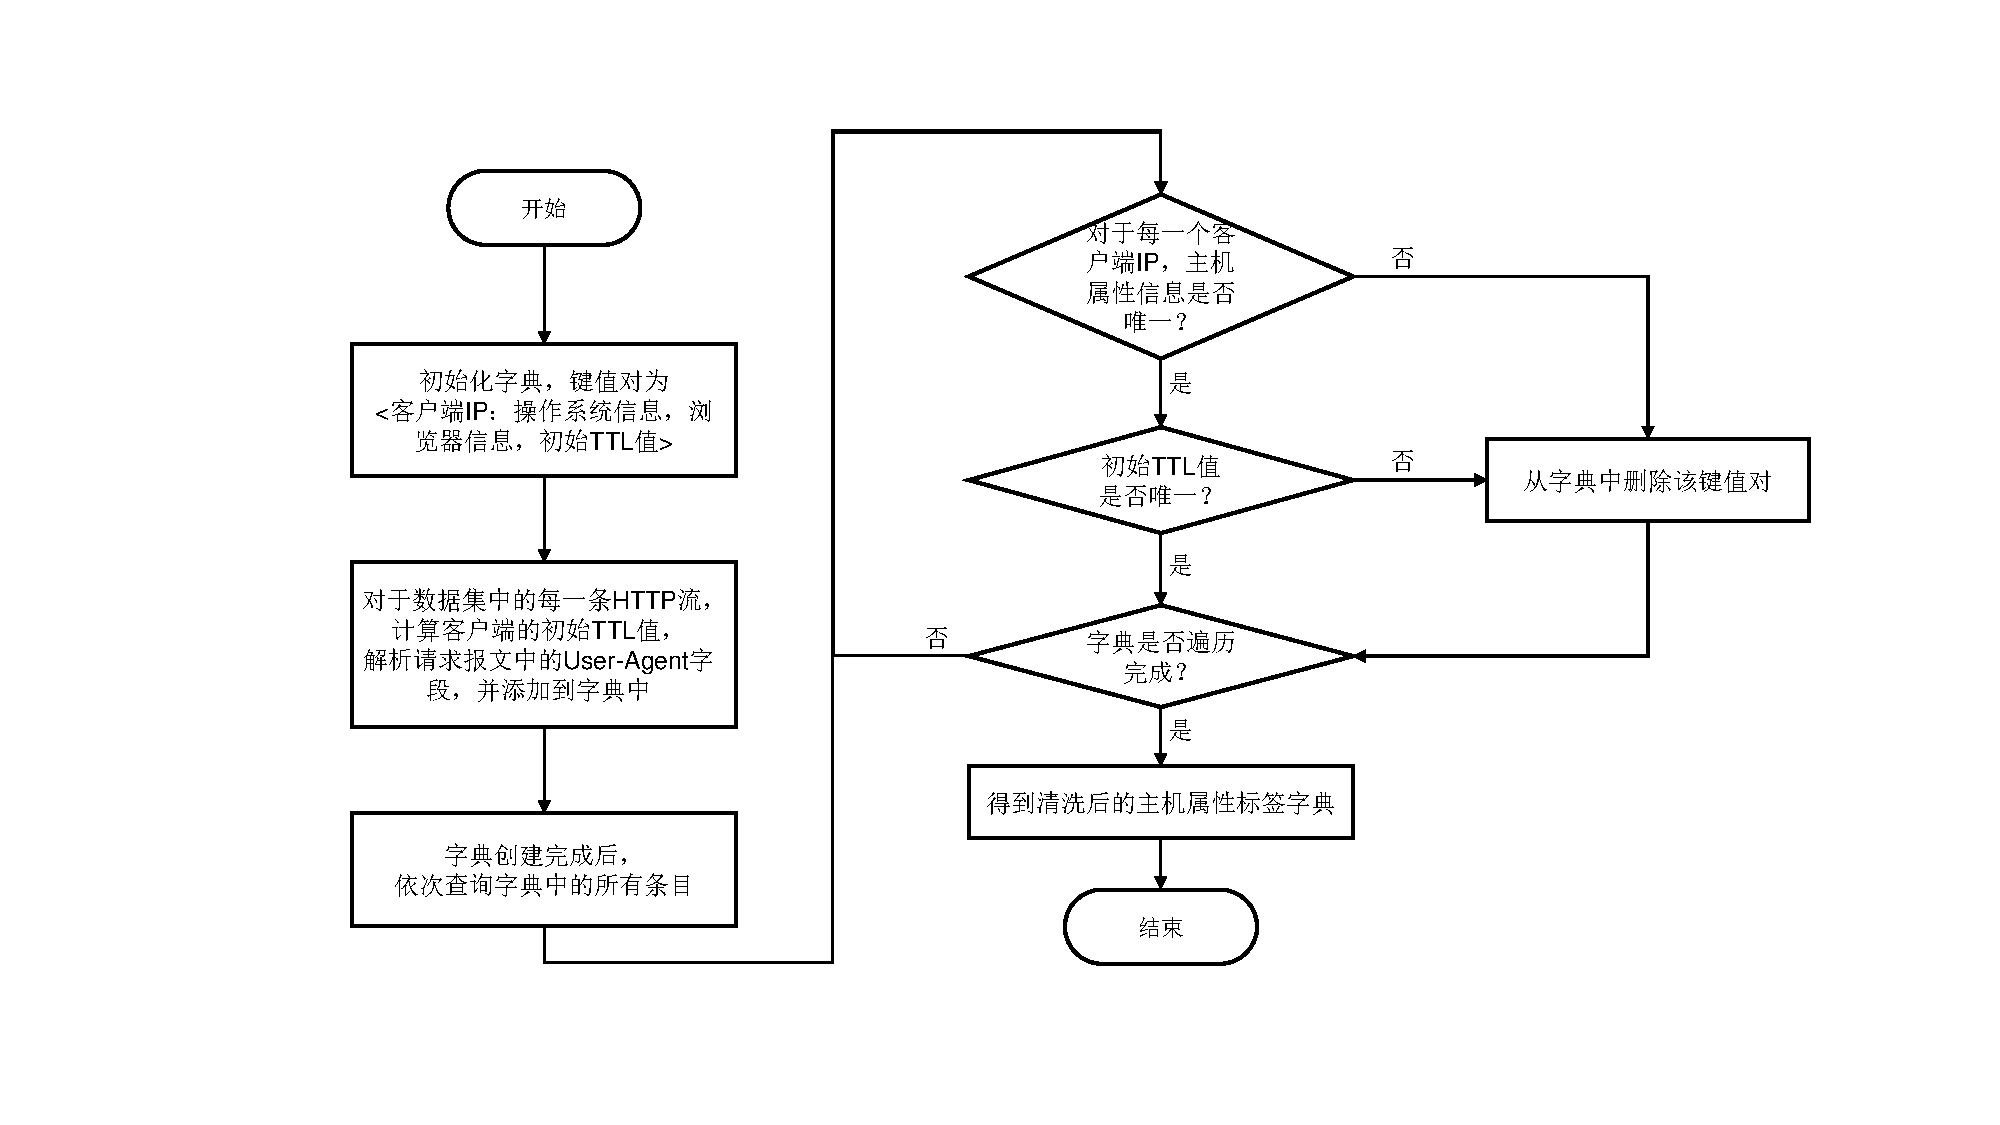
\includegraphics[width=0.9\textwidth]{属性标注方法}
    \bicaption{构建主机属性标签字典流程}{Build host attribute tag dictionary process}
\end{figure}

\subsection{数据集中的主机属性分布} 
经过统计,标注数据集中共包含了5种操作系统类型,21种操作系统主版本以及5种浏览器类型。操作系统类型主要有Android、iOS、Windows、MacOS以及Linux等,浏览器类型主要有Firefox、Safari、IE、Chrome以及Opera等。

在操作系统类型方面,如图3.7(a)所示,Android系统和Windows系统的设备数量最多,占比分别为53.3\%和37.7\%。其次是Apple公司的iOS系统和MacOS系统,共计占比约7.7\%。而Linux系统占比最少,仅为1.4\%。

如图3.7(b)所示,在各类操作系统主版本中,Android 6、Android 7、Android 8和Windows 7等系统版本的数量占比最多。此外,由于从HTTP协议的User-Agent字段中无法识别更多Linux系统的主版本信息,因此本文仅研究最流行的桌面Linux发行版即Ubuntu系统的是识别技术。

在浏览器属性方面,如图3.7(c)所示,谷歌公司的Chrome浏览器和Apple公司的Safari浏览器在数据集中占比最高。通过查阅相关资料,以上各类操作系统和浏览器类型在数据集中的分布基本符合其在国际上的市场份额占比状况。

\begin{figure}[!htbp]
    \centering
    \begin{subfigure}[b]{0.32\textwidth}
      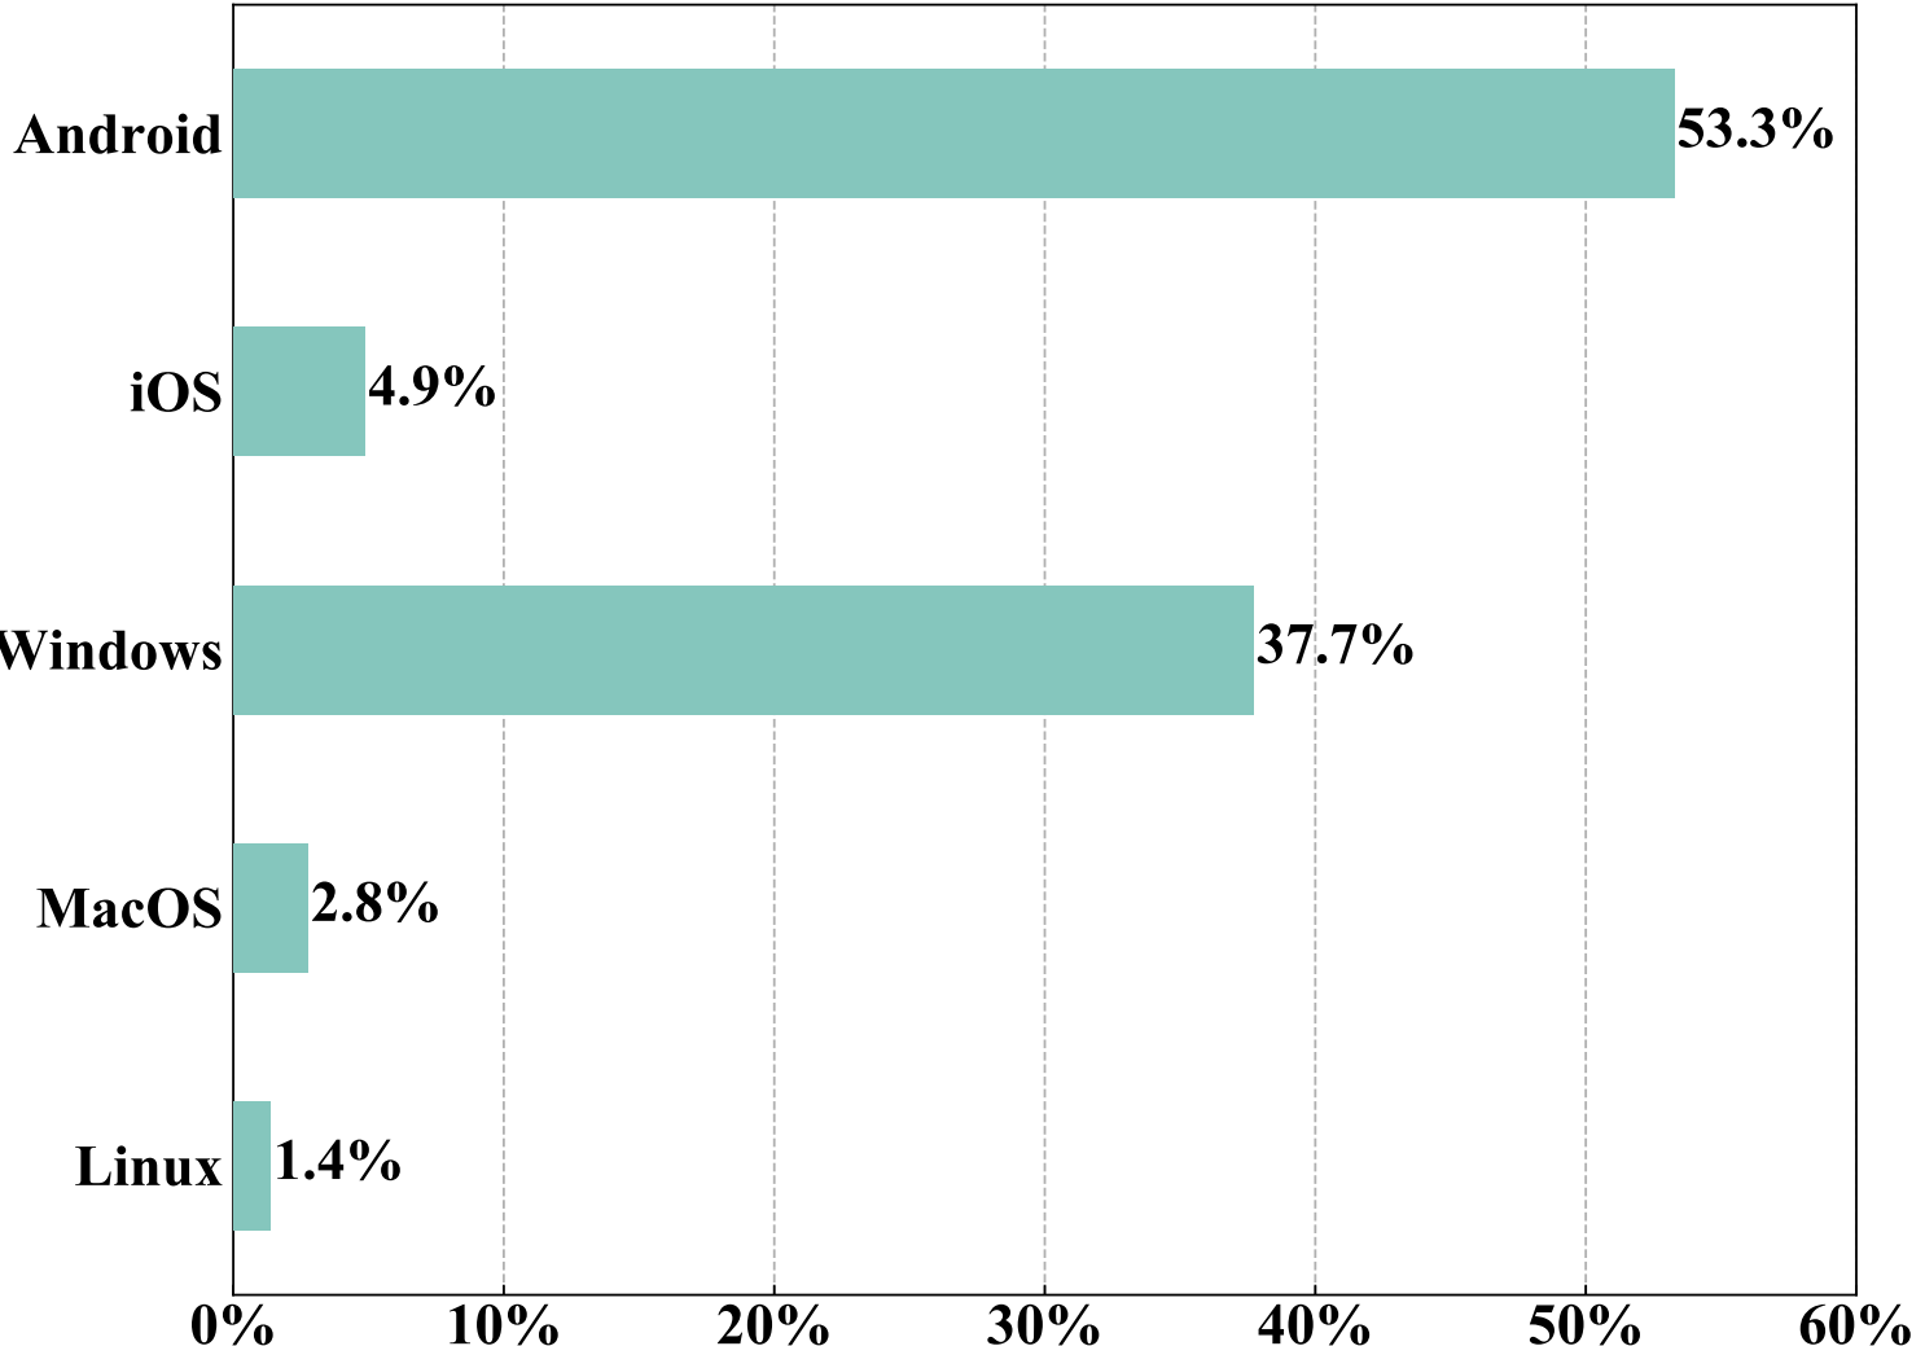
\includegraphics[width=\textwidth]{3-6-1}
      \caption{操作系统类型分布}
    \end{subfigure}%
    \hspace{10pt}
    \begin{subfigure}[b]{0.32\textwidth}
      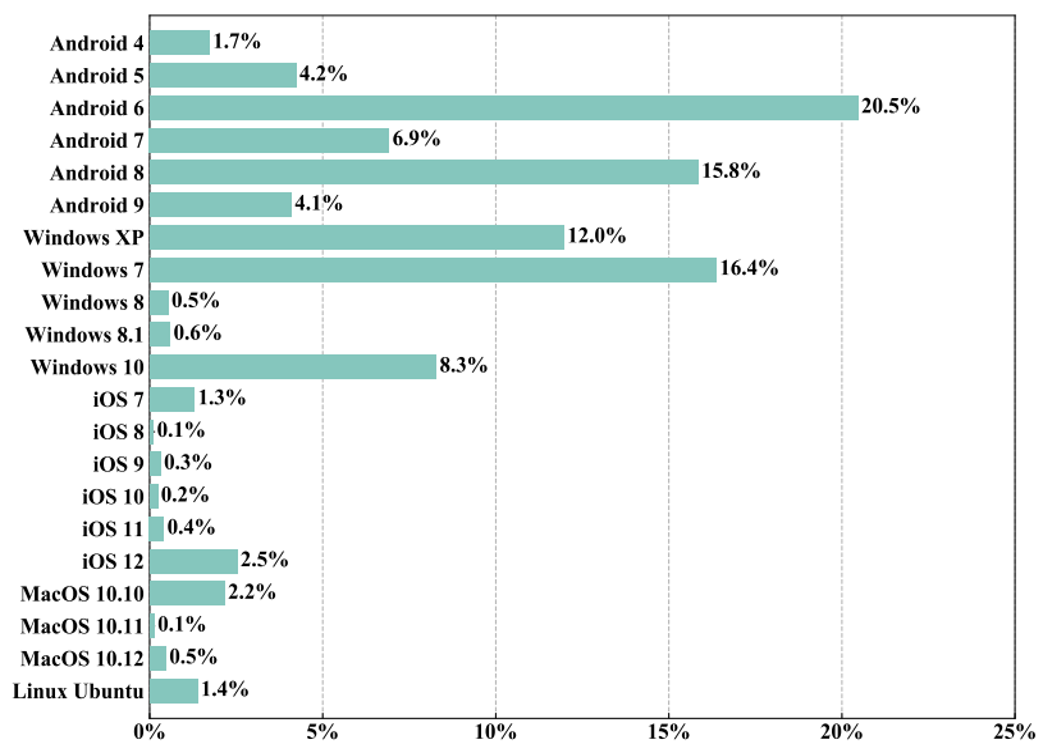
\includegraphics[width=\textwidth]{3-6-2}
      \caption{操作系统版本分布}
    \end{subfigure}
    \hspace{10pt}
    \begin{subfigure}[b]{0.29\textwidth}
      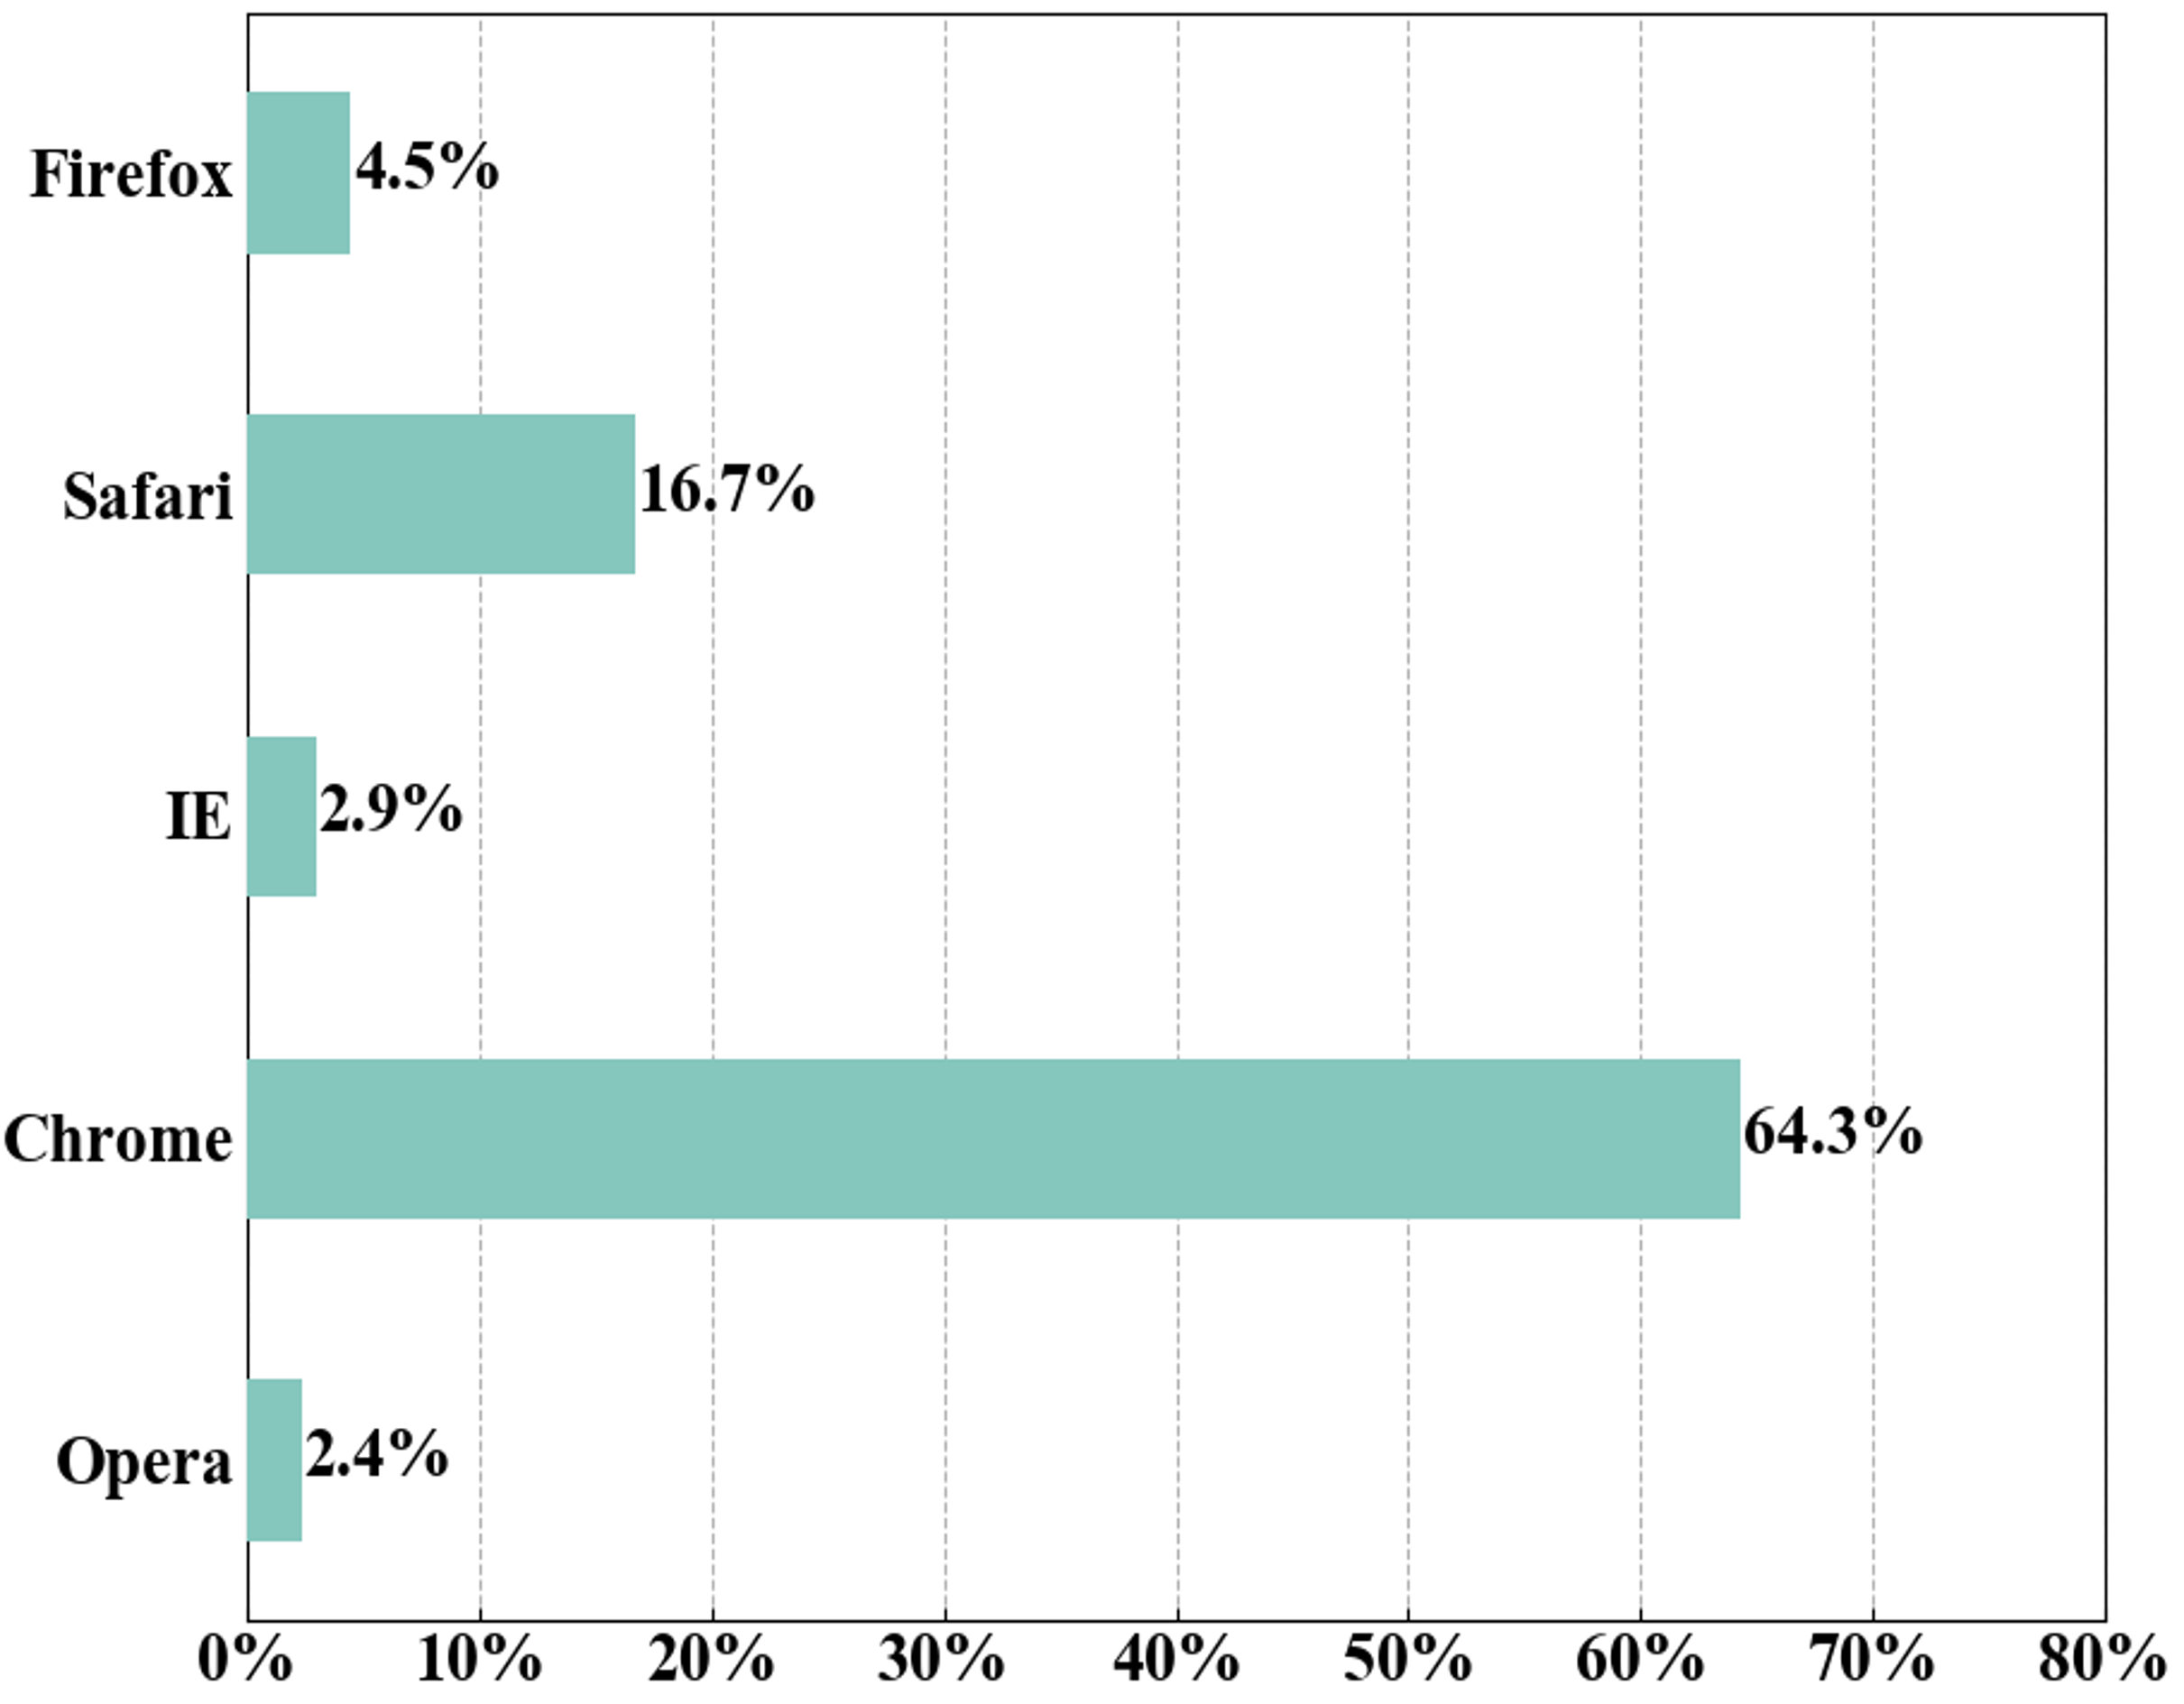
\includegraphics[width=\textwidth]{3-7}
      \caption{浏览器类型分布}
    \end{subfigure}  
    \centering  
    \bicaption{数据集中的主机属性分布(a)操作系统类型分布,(b)操作系统版本分布,(c)浏览器类型分布}{Distribution of host attributes in the dataset(a)Operating system type distribution, (b)Operating system version distribution, (c)Browser type distribution}
\end{figure}

\section{实验设计与结果分析}

\subsection{模型对比}

本节将分别测试3.3节中介绍的逻辑回归模型、最近邻居模型、随机森林模型、XGBoost模型以及LightGBM模型等五类机器学习模型在主机属性识别任务中的效果和性能。

若无特殊说明,本文所有实验都在同一环境中进行,以避免因机器性能不同带来的实验结果误差。实验环境的操作系统为Windows,CPU型号为Intel Core i7-7300HQ,GPU型号为GTX 1080Ti,内存大小为32GB,采用的编程语言为Python语言,调用的算法实现库为Sklearn库。

在对比实验中,本文采取的评估指标主要有准确率、精度、召回率、F1分数、PR曲线和模型预测速率。其中,F1分数是统计学中用来衡量分类模型精确度的一种指标。它同时兼顾了分类模型的准确率和召回率,可以看作是模型准确率和召回率的一种调和平均。

\begin{figure}[!h]
    \centering
    \begin{subfigure}[b]{0.8\textwidth}
      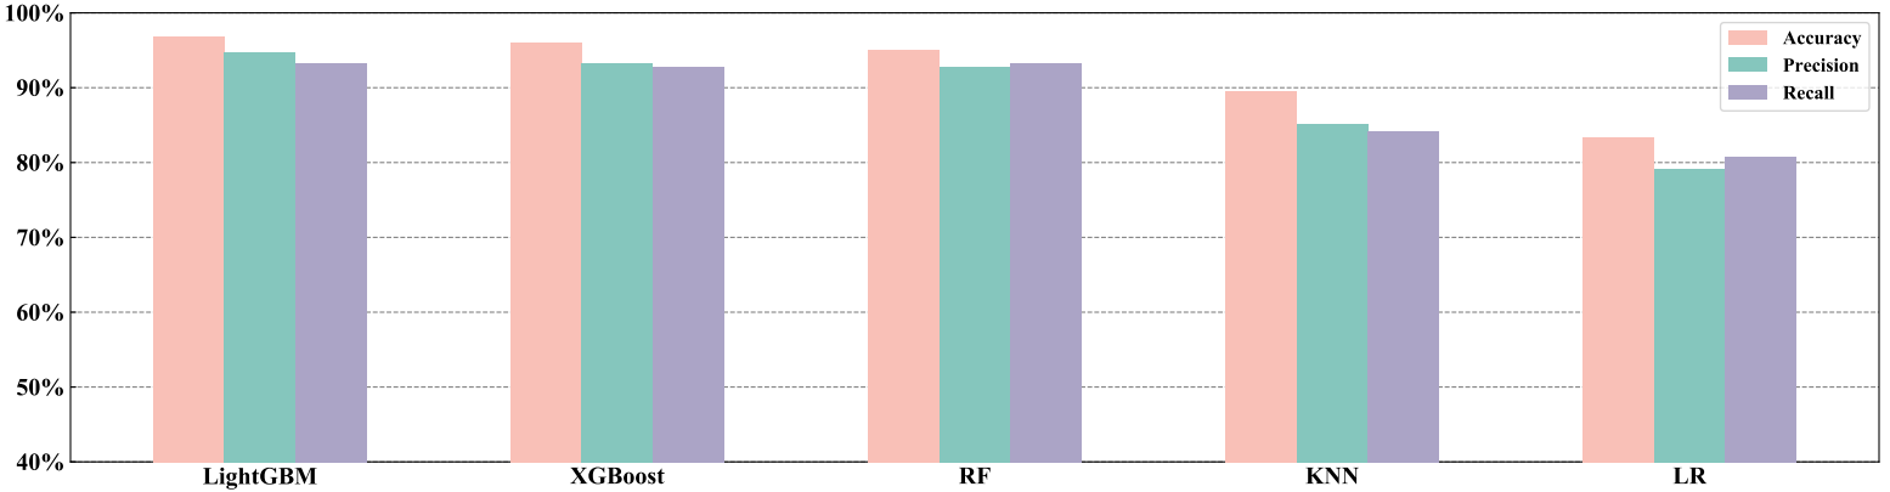
\includegraphics[width=\textwidth]{3-8-1}
      \caption{操作系统类型识别结果}
    \end{subfigure}
    \begin{subfigure}[b]{0.8\textwidth}
      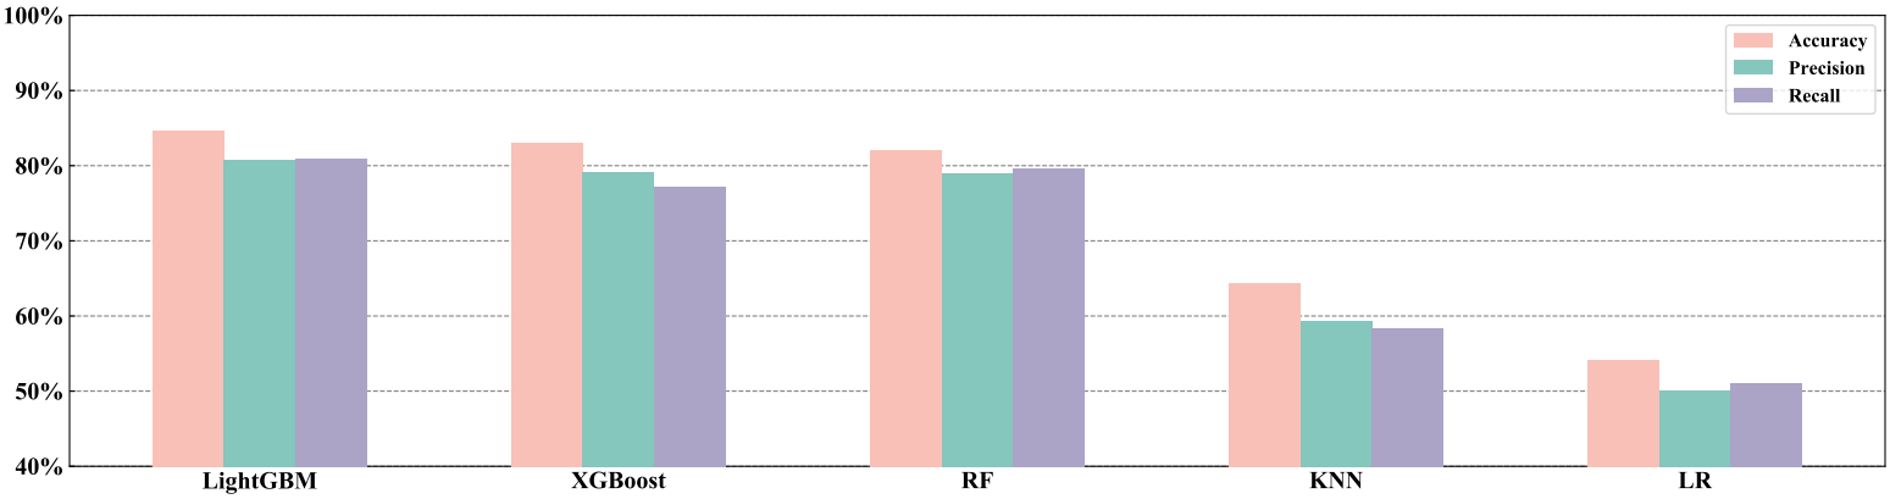
\includegraphics[width=\textwidth]{3-8-2}
      \caption{操作系统版本识别结果}
    \end{subfigure}
    \begin{subfigure}[b]{0.8\textwidth}
      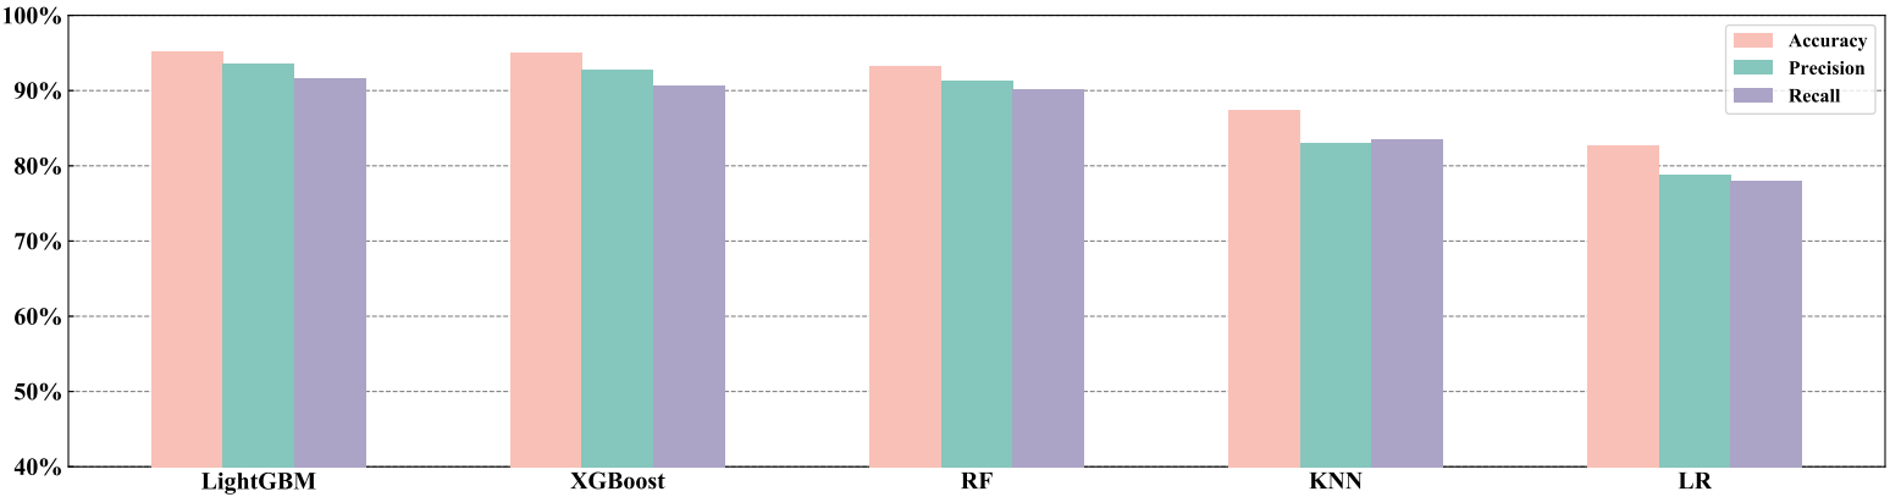
\includegraphics[width=\textwidth]{3-8-3}
      \caption{浏览器类型识别结果}
    \end{subfigure}
    \bicaption{识别任务准确率、精度以及召回率对比(a)操作系统类型识别结果,(b)操作系统版本识别结果,(c)浏览器类型识别结果}{Comparison of identification task accuracy, precision and recall(a)Operating system type identification results, (b)Operating system version identification results, (c)Browser type identification results}
    \label{fig:3-8}
\end{figure}

如图3.8所示,在准确率、精度以及召回率方面,LightGBM模型在所有识别任务中的表现均是最佳。在操作系统和浏览器的类型识别任务中,RF模型、XGBoost模型以及LightGBM模型的各项指标都在90\%以上,充分显示了集成树模型的优越性。在主机属性识别任务中,大部分输入特征均为类别特征,而树模型的分类策略对这种离散特征的适应性非常强,再经过集成模型对基学习器的效果改善,使得集成树模型较为适用于该识别任务。KNN模型和LR模型虽然三项指标都达到了80\%左右,但由于算法结构较为简单,更适合处理线性分类任务,在决策空间较为复杂的主机属性识别任务中效果较差。

\begin{figure}[!h]
    \centering
    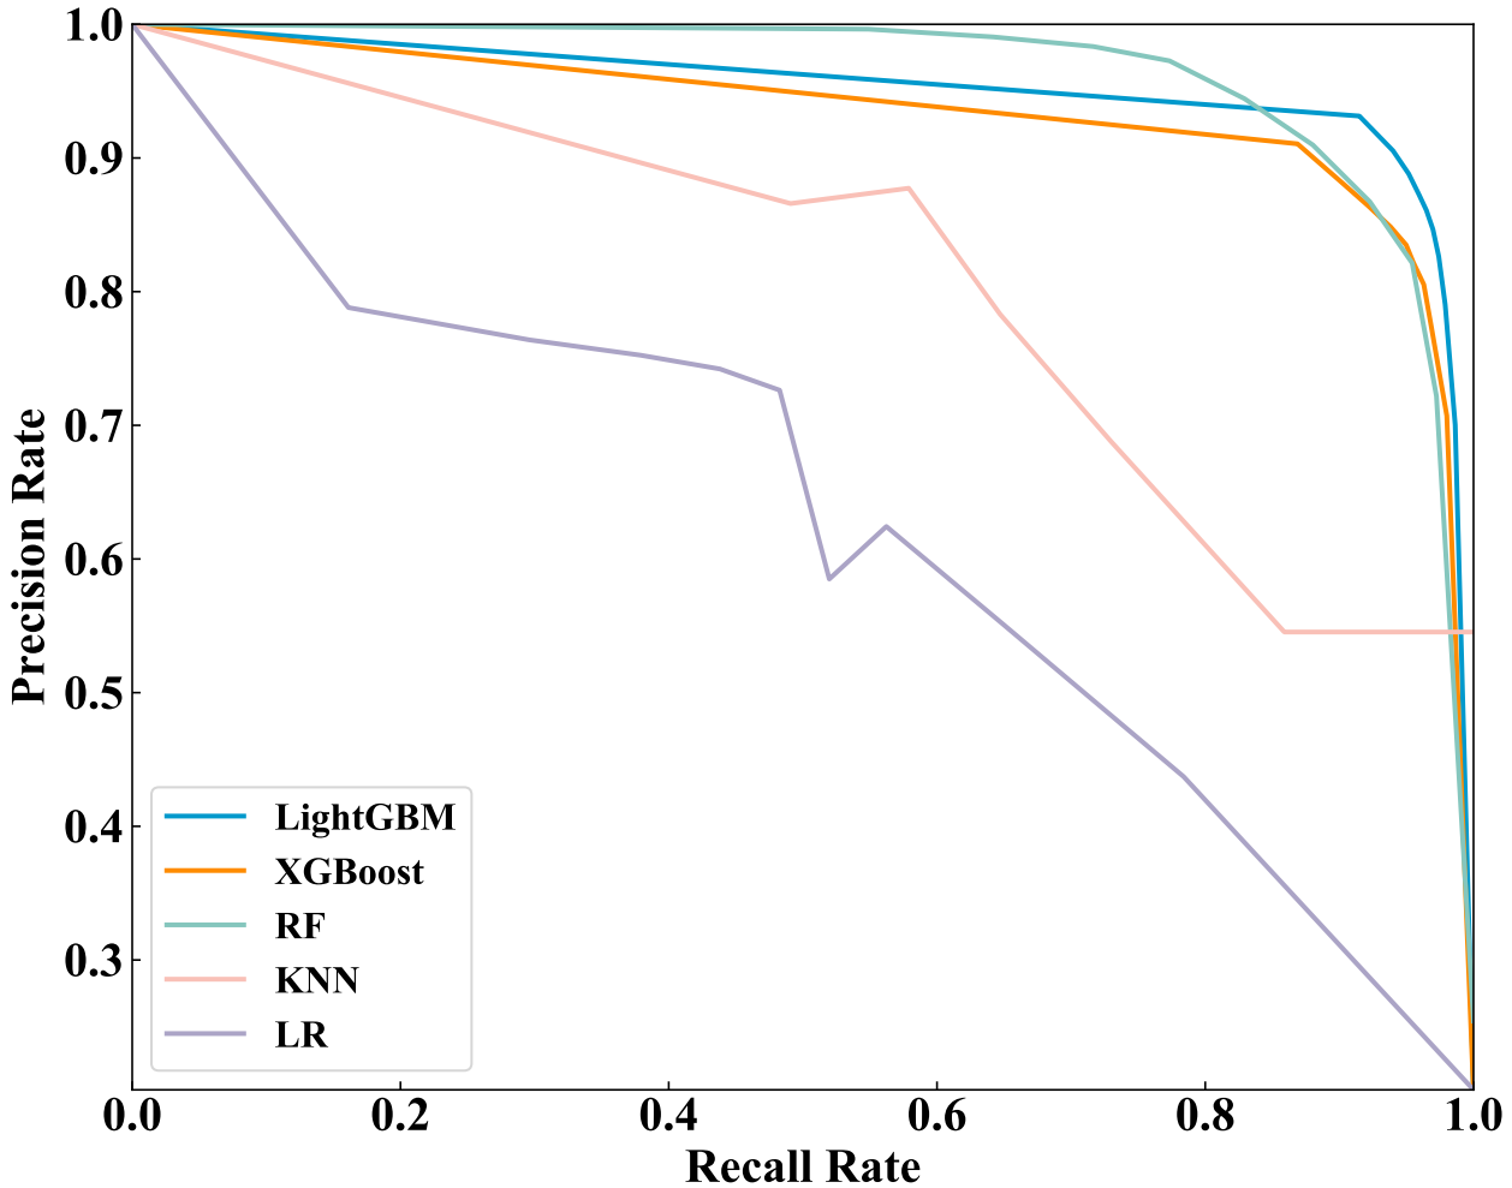
\includegraphics[width=0.6\textwidth]{3-9}
    \bicaption{操作系统版本识别任务PR曲线}{The PR curve of operating system version identification task}
    \label{fig:3-9}
\end{figure}

PR曲线是以召回率为横轴,以精度为纵轴绘制出的曲线,可以直观衡量一个模型的预测能力。在操作系统版本识别结果中,如图3.9所示,RF模型、XGBoost模型以及LightGBM模型的PR曲线均将KNN模型和LR模型的PR曲线完全包住,说明前三者的性能优于后者。而RF模型、XGBoost模型、LightGBM模型的PR曲线由于存在交叉点,不能根据以上标准分析优劣,但可以借助平衡点即召回率和精度相等的点比较性能。可以看到,LightGBM模型在平衡点处的值最大,说明该模型的性能更佳。

\begin{figure}[!h]
    \centering
    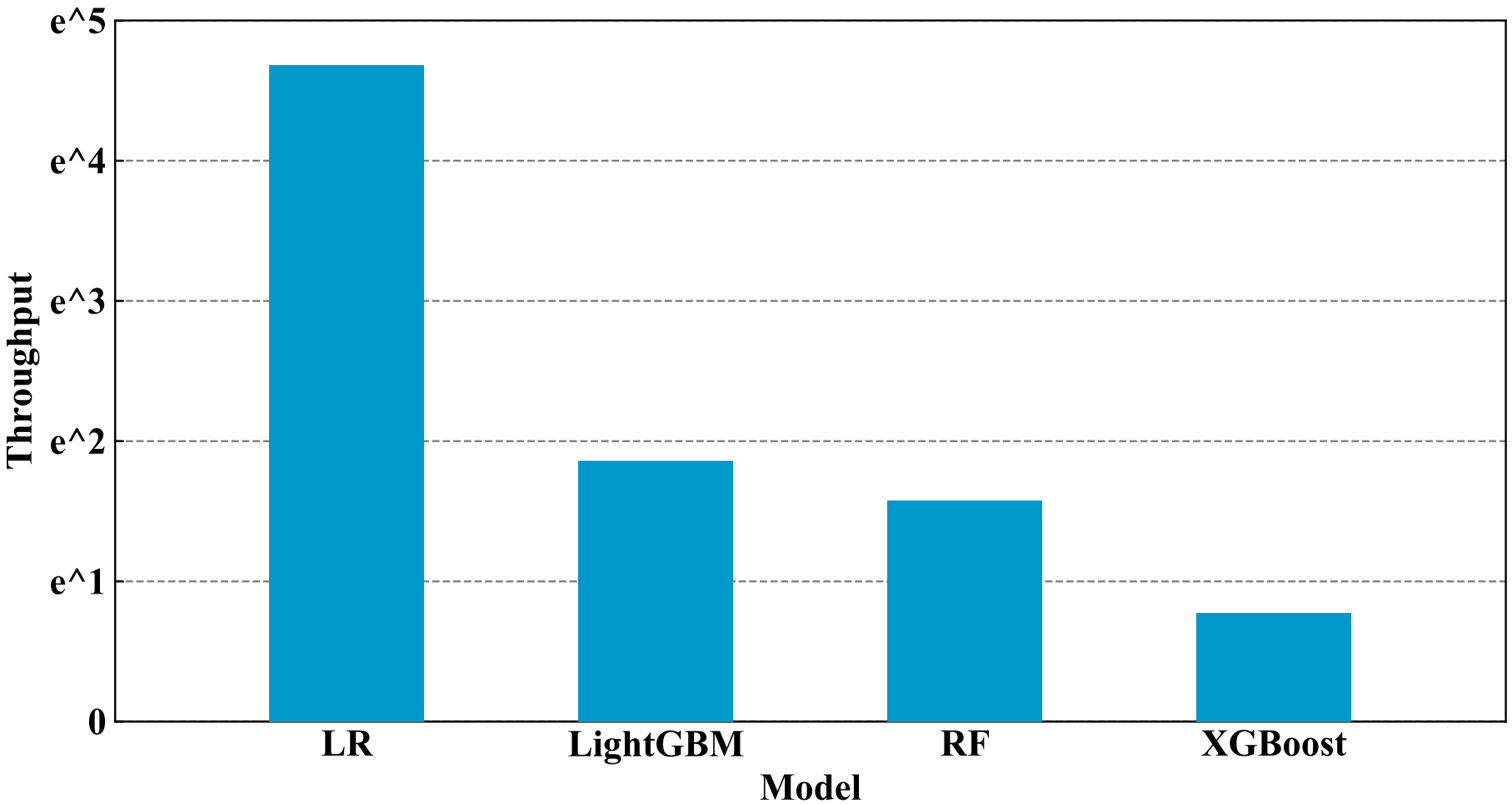
\includegraphics[width=0.8\textwidth]{3-10}
    \bicaption{操作系统版本识别任务吞吐量柱状图}{The throughput histogram of Operating system version identification task}
    \label{fig:3-10}
\end{figure}

通过分析在操作系统版本识别任务中的吞吐量可以得到各模型之间的预测速率差异。如图3.10所示,LR模型由于简单的分类策略,识别效率最高,比位于第二名的LightGBM模型快几十倍。在三类集成树模型中,LightGBM模型的预测速率最快,这主要是因为LightGBM模型采用直方图算法优化了树的生长速率,并对多线程任务进行了特殊优化,更适合多分类任务。对于KNN模型,由于独特的识别算法,其预测速率依赖于训练样本空间的规模,因此不适合在单一任务中与其他模型进行对比。

通过以上实验结果对比可以发现,LightGBM模型由于在GBDT算法的基础上进行了优化改进,在准确率、精度、召回率、PR曲线以及模型预测速率等方面的表现都较为优越。因此,本章采用LightGBM模型作为主机属性发现任务中的最终模型。

\subsection{泛化性能评估}

为了验证模型的泛化性能,本节将数据集按照日期进行切分,以前四天的数据作为训练集,最后一天的数据作为测试集,比较LightGBM模型在两个数据集上的性能差异。

图3.11展示了LightGBM模型在操作系统类型识别任务中的识别结果。从柱状图中可以看到,模型在训练集和测试集中的识别结果差异性非常小,准确率、精度以及召回率的最大差异不超过1\%。在折线图中,LightGBM模型识别每一类操作系统的精度和召回率变化同样较小。由此说明,基于协议字段特征和流统计特征的LightGBM模型具备很强的泛化能力。

\begin{figure}[!htbp]
    \centering
    \begin{subfigure}[b]{0.33\textwidth}
      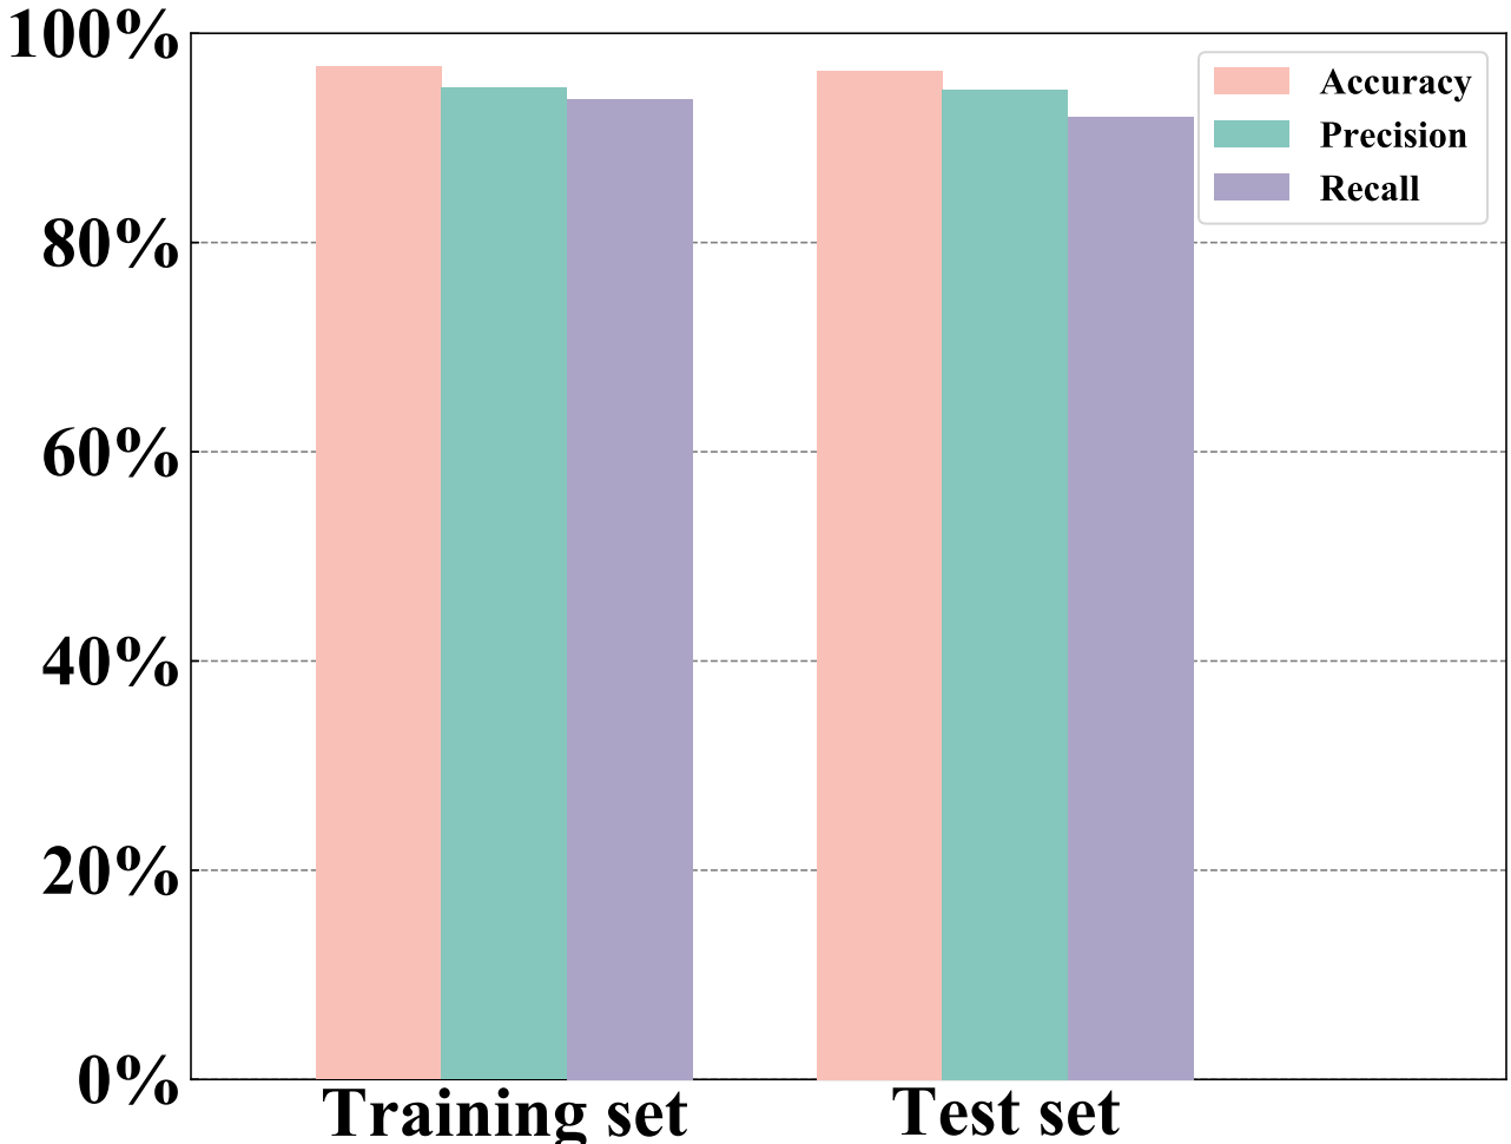
\includegraphics[width=\textwidth]{3-11-1}
      \caption{准确率、精度和召回率柱状图}
    \end{subfigure}%
    \hspace{20pt}
    \begin{subfigure}[b]{0.4\textwidth}
      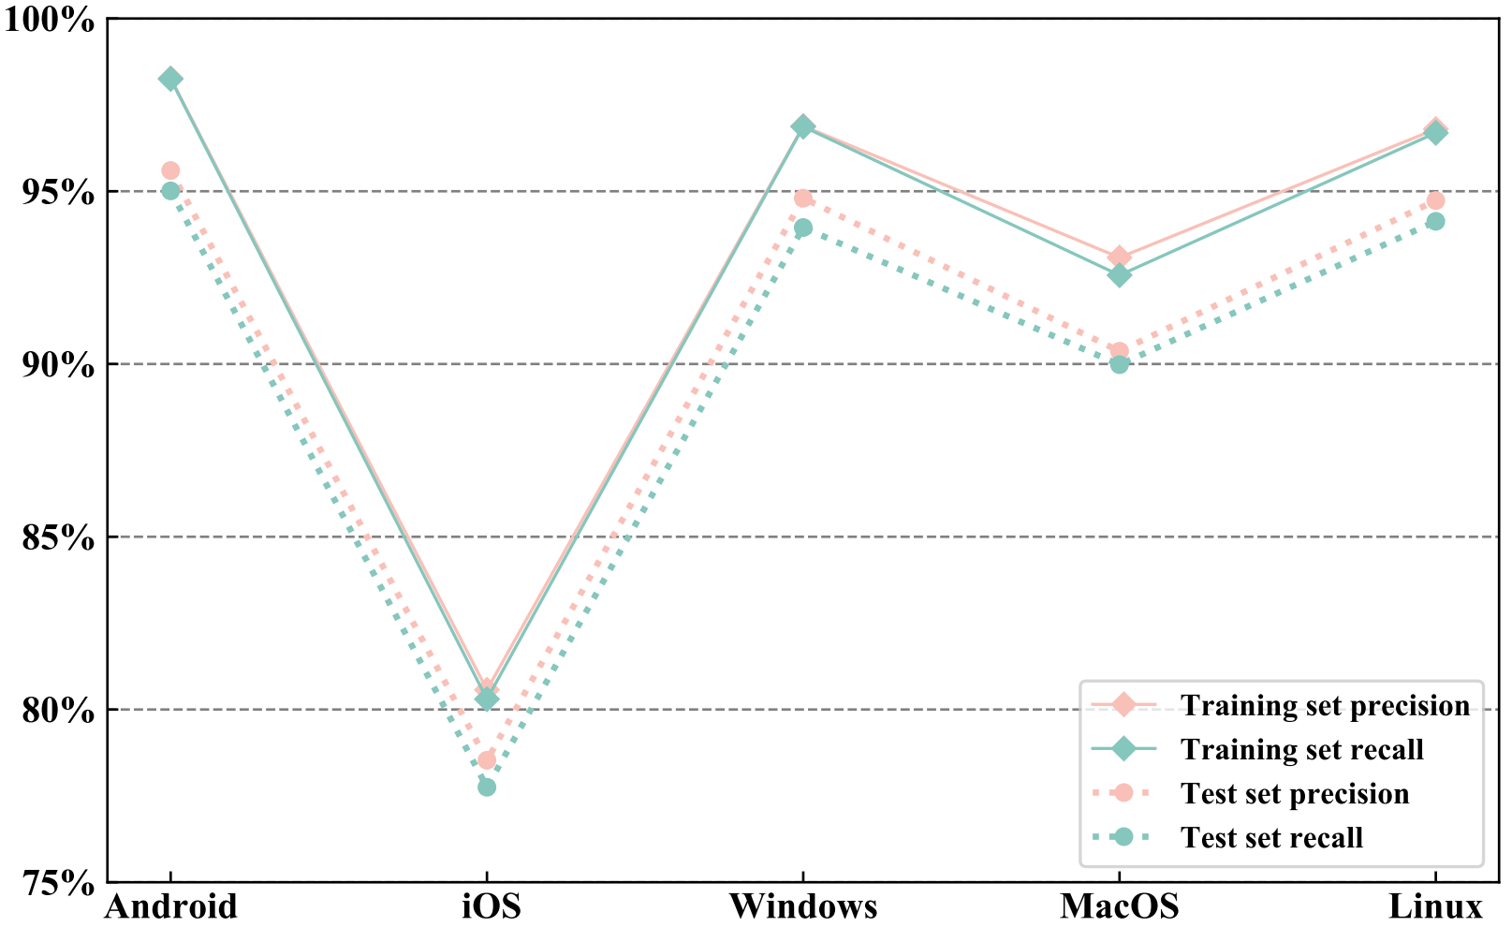
\includegraphics[width=\textwidth]{3-11-2}
      \caption{精度和召回率折线图}
    \end{subfigure}
    \bicaption{操作系统类型识别(a)准确率、精度和召回率柱状图,(b) 精度和召回率折线图}{Operating system type identification results(a)Histogram of accuracy, precision and recall, (b)Line chart of accuracy and recall}
    \label{fig:3-11}
\end{figure}

\subsection{主机属性识别结果}

通过以上实验对比,不难发现LightGBM模型在众多机器学习模型中拥有最优的表现。因此,本章基于13维协议字段特征和上百维流统计特征,结合LightGBM模型,提出了开放环境中的细粒度主机属性发现技术,可以高效、精准地识别加密网络中客户端主机的多维属性。利用该技术对数据集中的所有样本进行主机属性识别,可得结果如表3.7-3.9所示。

在操作系统类型识别任务中,分类器在测试集上的识别准确率达到了96.29\%,F1值也高达91.53\%。其中,Android系统的识别效果最好,精度为98.27\%,比平均值高了5\%左右,这主要是因为主机属性识别任务是一个类别不均衡任务,Android系统对应的样本量在数据集中最多,导致学习器在训练过程中对其有所偏好。Linux系统和Windows系统的识别效果次之,MacOS系统和iOS系统的识别效果最差,这是因为iOS系统和MacOS系统同属于一家厂商,其网络协议栈指纹的相似性较高,导致在识别过程中容易混淆。

\begin{table}[!h]
    \bicaption{操作系统类型识别结果}{Operating system type identification results}
    \centering
    \footnotesize
    \setlength{\tabcolsep}{8pt}
    \renewcommand{\arraystretch}{1}
\begin{tabular}{|c|c|c|c|c|c|c|c|}
\hline
\multirow{2}{*}{\textbf{ID}} & \multirow{2}{*}{\textbf{操作系统类型}} & \multicolumn{3}{c|}{\textbf{训练集}} & \multicolumn{3}{c|}{\textbf{测试集}} \\ \cline{3-8} 
 &  & \textbf{Precision} & \textbf{Recall} & \textbf{F1} & \textbf{Precision} & \textbf{Recall} & \textbf{F1}\\ \hline
1 & Android & 98.27\% & 95.60\% & 96.92\% & 98.25\% & 95.01\% & 96.60\% \\ \hline
2 & iOS & 80.57\% & 78.53\% & 79.54\% & 80.30\% & 77.75\% & 79.00\% \\ \hline
3 & Windows & 96.89\% & 94.80\% & 95.83\% & 96.87\% & 93.95\% & 95.39\% \\ \hline
4 & MacOS & 93.08\% & 90.37\% & 91.70\% & 92.57\% & 89.98\% & 91.26\% \\ \hline
5 & Linux & 96.80\% & 94.73\% & 95.75\% & 96.69\% & 94.13\% & 95.39\% \\ \hline
\multicolumn{2}{|c|}{\textbf{AVE}} & 93.12\% & 90.81\% & 91.95\% & 92.94\% & 90.16\% & 91.53\% \\ \hline
\multicolumn{2}{|c|}{\textbf{Accuracy}} & \multicolumn{3}{c|}{96.89\%} & \multicolumn{3}{c|}{96.29\%} \\ \hline
\end{tabular}
\end{table}

\begin{table}[!h]
    \bicaption{操作系统版本识别结果}{Operating system version identification results}
    \centering
    \footnotesize
    \setlength{\tabcolsep}{8pt}
    \renewcommand{\arraystretch}{1}
\begin{tabular}{|c|c|c|c|c|c|c|c|}
\hline
\multirow{2}{*}{\textbf{ID}} & \multirow{2}{*}{\textbf{操作系统版本}} & \multicolumn{2}{c|}{\textbf{测试集}} & \multirow{2}{*}{\textbf{ID}} & \multirow{2}{*}{\textbf{操作系统版本}} & \multicolumn{2}{c|}{\textbf{测试集}} \\ \cline{3-4} \cline{7-8}
 &  & \textbf{Precision} & \textbf{Recall} & & & \textbf{Precision} & \textbf{Recall} \\ \hline
1 & Android 4 & 81.23\% & 66.27\% & 12 & iOS 7 & 99.44\% & 99.36\% \\\hline
2 & Android 5 & 71.44\% & 60.67\% & 13 & iOS 8 & 70.58\% & 86.04\% \\\hline
3 & Android 6 & 94.64\% & 87.23\% & 14 & iOS 9 & 72.18\% & 80.84\% \\\hline
4 & Android 7 & 89.27\% & 59.85\% & 15 & iOS 10 & 51.45\% & 69.11\% \\\hline
5 & Android 8 & 67.07\% & 88.97\% & 16 & iOS 11 & 49.80\% & 69.10\% \\\hline
6 & Android 9 & 63.72\% & 42.41\% & 17 & iOS 12 & 57.36\% & 85.79\% \\\hline
7 & Windows XP & 98.30\% & 94.11\% & 18 & MacOS 10 & 99.26\% & 94.89\% \\\hline
8 & Windows 7 & 91.08\% & 95.07\% & 19 & MacOS 11 & 88.67\% & 66.50\% \\\hline
9 & Windows 8 & 78.87\% & 43.36\% & 20 & MacOS 12 & 81.45\% & 64.82\% \\\hline
10 & Windows 8.1 & 90.99\% & 57.74\% & 21 & Ubuntu & 94.44\% & 95.38\% \\\hline
11 & Windows 10 & 89.19\% & 88.22\% & \multicolumn{2}{c|}{\textbf{AVE}} & 80.02\% & 75.99\% \\\hline
\end{tabular}
\end{table}

操作系统版本识别任务属于细粒度主机属性识别任务,在表3.8所示的实验结果中,可以看到细粒度主机属性的识别效果有所降低,平均的识别精度和召回率分别未80.02\%和75.99\%。通过观察识别结果的混淆矩阵,如图3.12所示,可以发现许多相邻版本的操作系统相互之间很容易产生识别混淆,这主要是因为部分操作系统在版本更新时,对网络协议栈的具体实现改动不多,导致其流量特征的可区分性不足,从而降低了分类器的识别准确性。


\begin{figure}[!h]
    \centering
    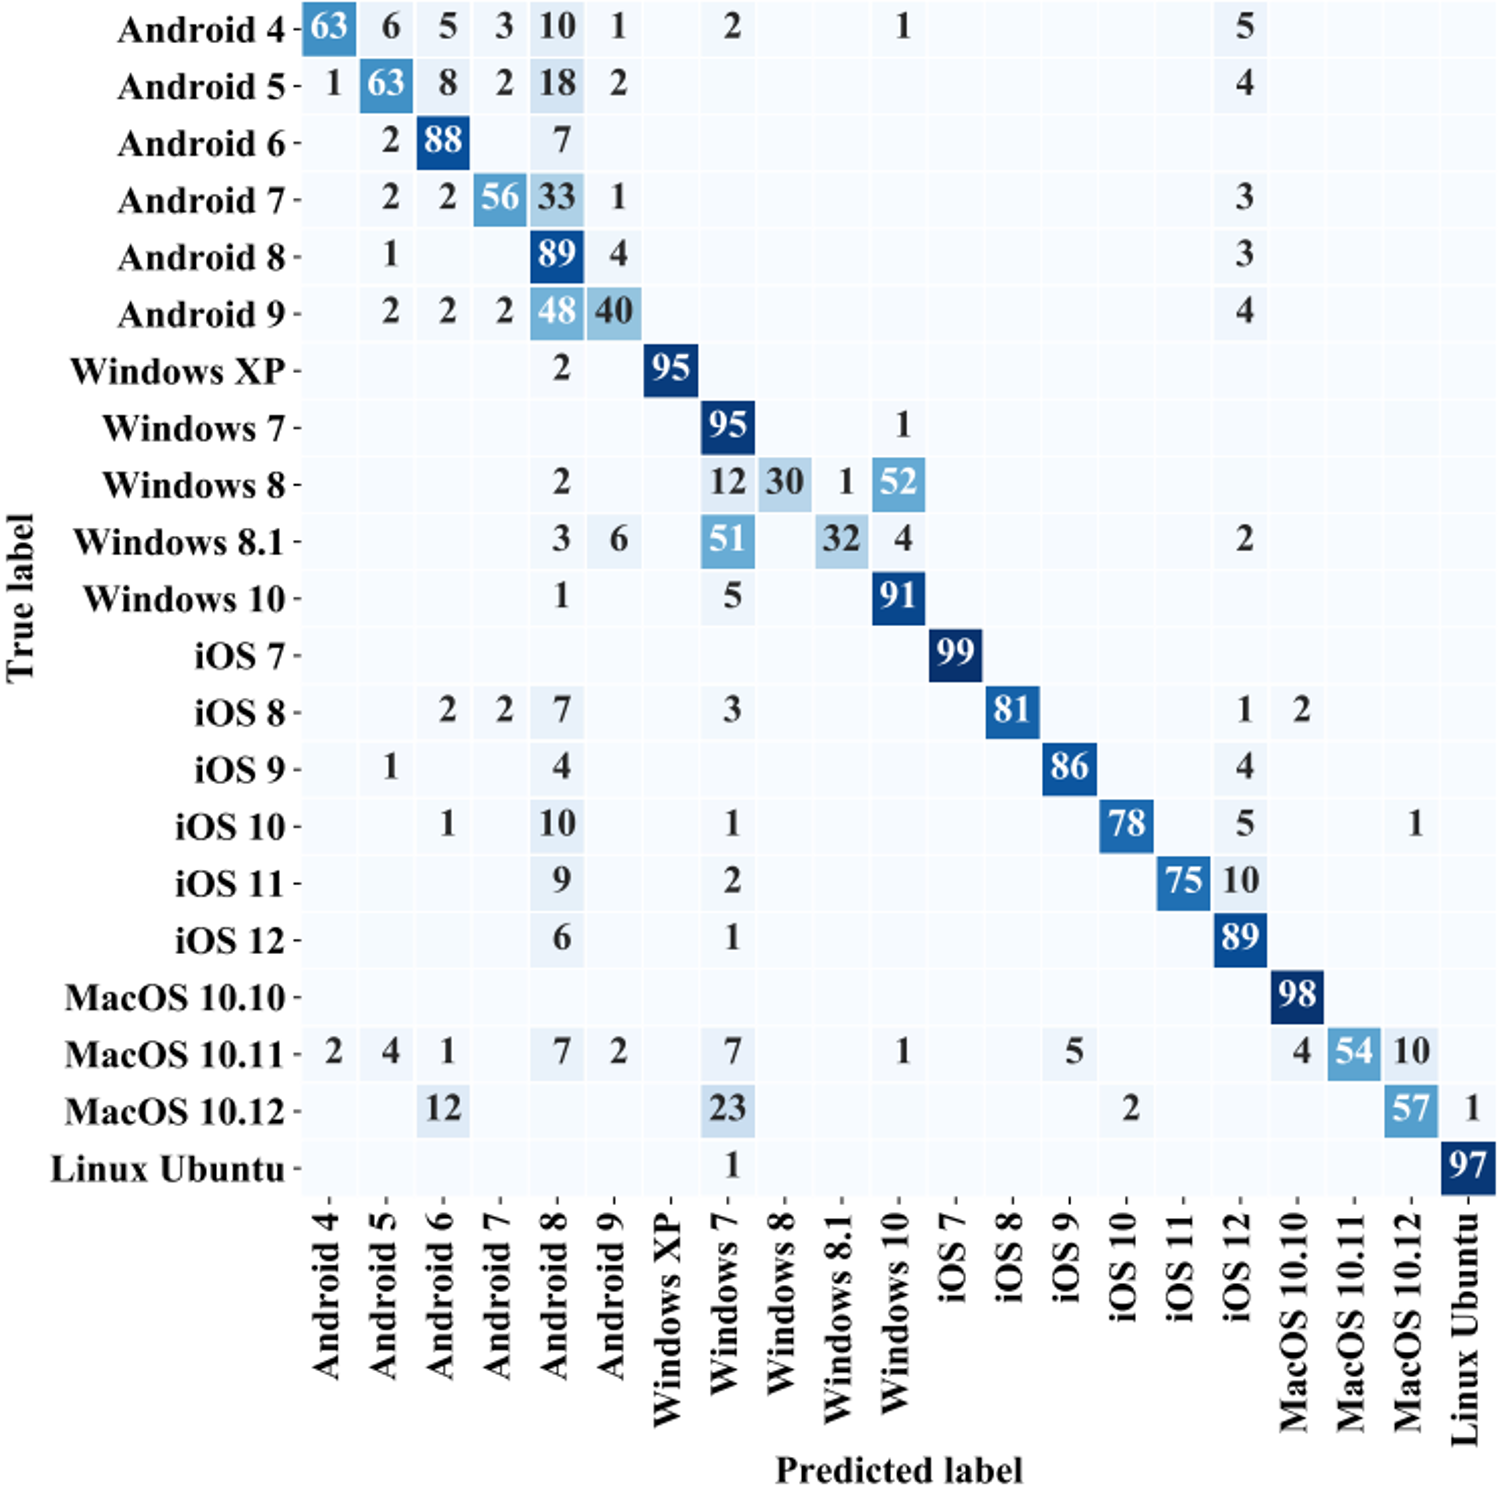
\includegraphics[width=0.7\textwidth]{3-12}
    \bicaption{操作系统版本识别任务混淆矩阵}{The confusion matrix of operating system version identification task}
    \label{fig:3-12}
\end{figure}

\vbox{}
在浏览器类型识别任务中,测试集的识别准确率和F1值分别为94.02\%和91.50\%,识别效果较好。其中,由于Firefox浏览器的TCP/IP协议栈指纹变化较少,拥有最佳的识别效果,而Chrome浏览器和Safari浏览器因为多平台支持和较频繁的版本更新,识别效果偏差。

\begin{table}[!htbp]
    \bicaption{浏览器类型识别结果}{Browser type identification results}
    \centering
    \footnotesize
    \setlength{\tabcolsep}{8pt}
    \renewcommand{\arraystretch}{1}
\begin{tabular}{|c|c|c|c|c|c|c|c|}
\hline
\multirow{2}{*}{ \textbf{ID}} & \multirow{2}{*}{ \textbf{浏览器类型}} & \multicolumn{3}{c|}{ \textbf{训练集}} & \multicolumn{3}{c|}{ \textbf{测试集}} \\ \cline{3-8} 
 &  &  \textbf{Precision} &  \textbf{Recall} &  \textbf{F1} & \textbf{Precision} &  \textbf{Recall} &  \textbf{F1} \\ \hline
1 & Firefox & 96.22\% & 93.31\% & 94.74\% & 94.09\% & 93.03\% & 93.56\%\\ \hline
2 & Safari & 90.25\% & 90.15\% & 90.20\% & 89.63\% & 89.17\% & 89.40\%\\ \hline
3 & IE & 94.45\% & 92.77\% & 93.60\% & 94.23\% & 91.47\% & 92.83\% \\ \hline
4 & Chrome & 90.37\% & 87.57\% & 88.95\% & 89.76\% & 87.60\% & 88.67\%\\ \hline
5 & Opera & 94.31\% & 92.55\% & 93.42\% & 94.44\% & 91.73\% & 93.07\%\\ \hline
\multicolumn{2}{|c|}{\textbf{AVE}} & 93.12\% & 91.27\% & 92.18\% & 92.43\% & 90.60\% & 91.50\%\\ \hline
\multicolumn{2}{|c|}{\textbf{Accuracy}} & \multicolumn{3}{c|}{94.89\%} & \multicolumn{3}{c|}{94.02\%} \\ \hline
\end{tabular}
\end{table}


\section{本章小结}

本章介绍了一种可在开放环境中识别细粒度主机属性的技术方法。该方法基于加密流量中的TLS会话数据,以双向网络流为单位,提取TCP/IP协议栈指纹,包括IP层的跳数、包长、分片标识等字段,TCP层的传输窗口大小、窗口缩放因子、最大报文长度等字段以及TLS层的版本、扩展长度、密钥算法套件序列等字段,再结合对应流的包长序列、时间序列和速率等统计特征,并将训练后的LightGBM模型作为分类器,可以从加密网络中被动识别主机的操作系统类型、版本和浏览器类型等主机属性。实验结果表明,本方法拥有较高的识别准确率、召回率和计算效率,并且泛化性能同样十分优秀。
